\newpage 
\section{Consistency Models}
\subsection{Introduction}

Moving on from consensus models, which handle agreement on data values,
we now shift our focus to the ordering of operations and their validity:

\begin{Def}[Consistency Model]

    Within a distributed system, a consistency model acts as a contract 
    between systems on valid operation ordering (e.g., reads or writes) on shared data within the network.\\

    \noindent
    These models are critical for ensuring that a system behaves as expected when 
    replicating data across multiple nodes. \hfill \cite{scylladbConsistencyModels}
\end{Def}

\begin{Def}[Global Total Order]
    
    A Global Total Order is a sequence of operations that is agreed upon by all nodes in a distributed system.
    This means that such sequence given some client inputs, could reproduce the same state on a single machine.
\end{Def}

\noindent
Now we begin to list some common consistency models:

\begin{Def}[Strong Consistency]
    
    The client observes that all nodes \textit{appear} to agree on the order of execution. This means 
    all node reads of shared data are identical
    (Global Total Order of operations).
\end{Def}
\begin{Def}[Weak Consistency]
    
    The client \textbf{temporarily} observes that nodes disagree on shared data values at some point in time (no Global Total Order).
\end{Def}

\begin{theo}[Strong Consistency vs Weak Consistency]
    
    Even though strong consistency is desirable, it can be costly on the network and difficult to implement.
    Weak consistency is easier to implement and may provide better performance, but at the cost of data integrity and difficulty in debugging interactions.
\end{theo}
\newpage 

\noindent
Consider this example interaction, which interaction has the weakest consistency model?

\begin{figure}[h]
    \centering
    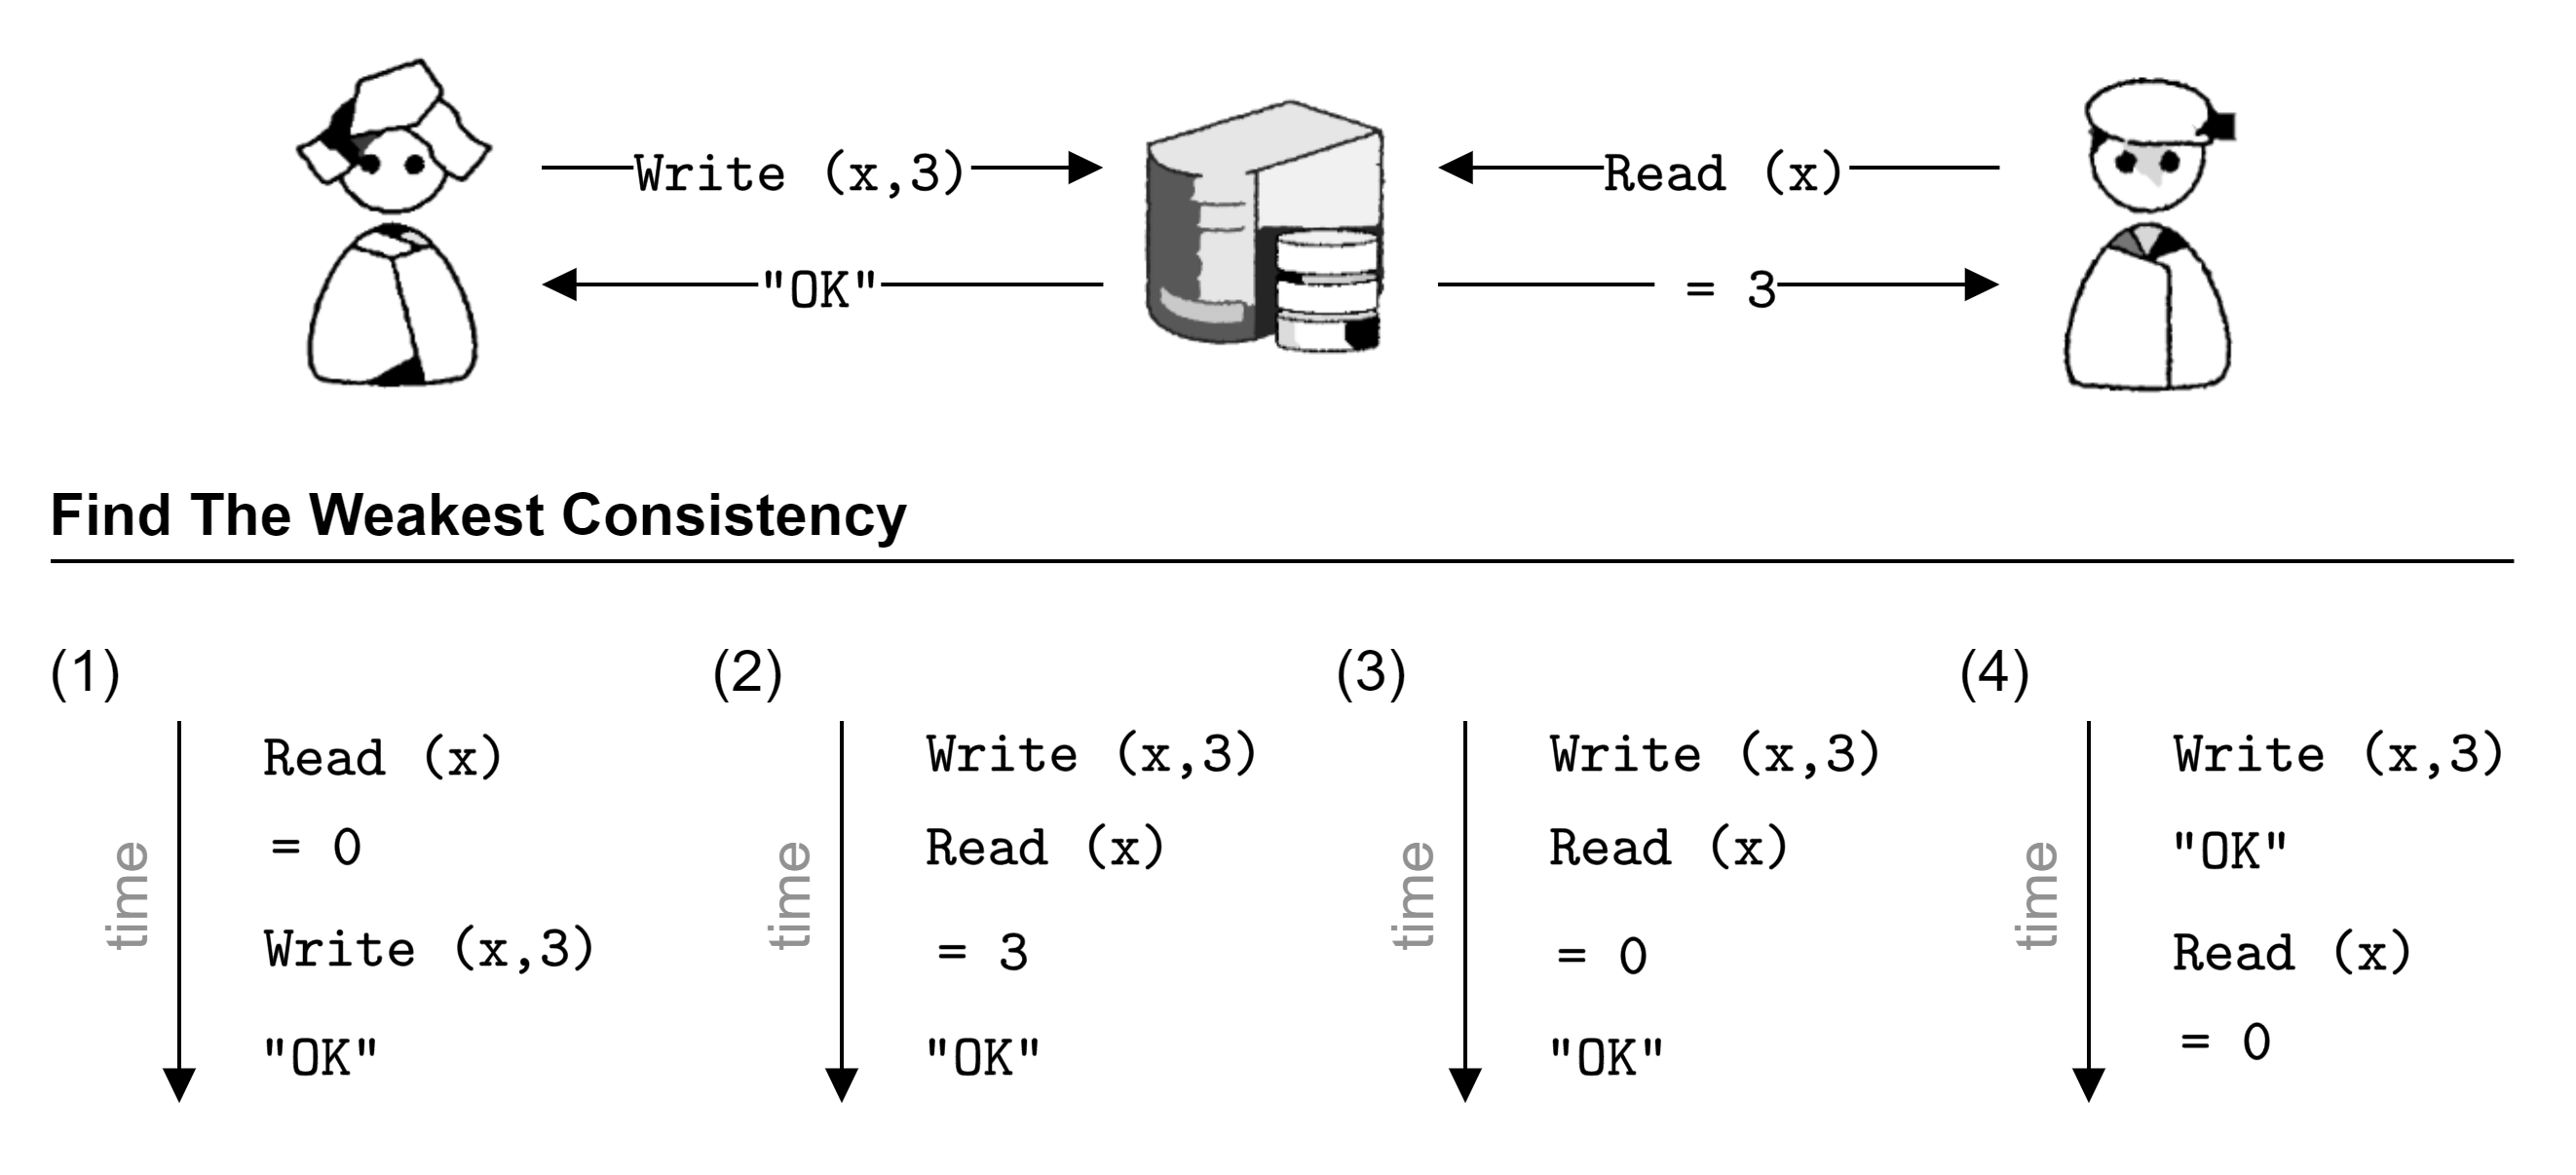
\includegraphics[width=\textwidth]{Sections/consist/consist.png}
    \caption{(1) Strong Consistency, as the read $x$ could be 0, and the write responds with ``OK''. (2) This is okay, as our write of 3 is read. The ``OK'' does come a little late, but its order isn't bizarre. (3) Still okay, as the ``OK'' comes after the read of 0, meaning the write could not have happened yet. (4) The weakest, as our read completely disregards our acknowledged write of 3.}
\end{figure}

\vspace{-1em}
\subsection{Strong Consistency Models: Linearizability \& Sequential Consistency}

We discuss two strong consistency models, Linearizability and Sequential Consistency:

\begin{Def}[Linearizability]
    
   Replicas produce a Global Total Order, which preserves real-time ordering of events.
   Moreover, every read must return the value of the \textbf{most completed} write. In particular:
   \begin{itemize}
    \item If operation $A$ completes before $B$, then $A\rightarrow B$ in real-time.
    \item If tasks $A$ and $B$ overlap, there is no real-time ordering.
   \end{itemize}
\end{Def}

\vspace{-.5em}
\begin{theo}[Raft and Linearizability]
    
    Raft's leader-commit design provides Linearizability, \textbf{except} in specific scenarios such as:
    \begin{itemize}
        \item A committed log entry is lost within the majority of the cluster.
        \item The newly elected leader somehow bypasses the Leader Completeness property.
    \end{itemize}

    \noindent
    In all other cases, Raft is considered to have a strong consistency model.
\end{theo}

\newpage

\noindent
Consider the following examples and determine whether it is linearizable:

\begin{figure}[h]
    \centering
    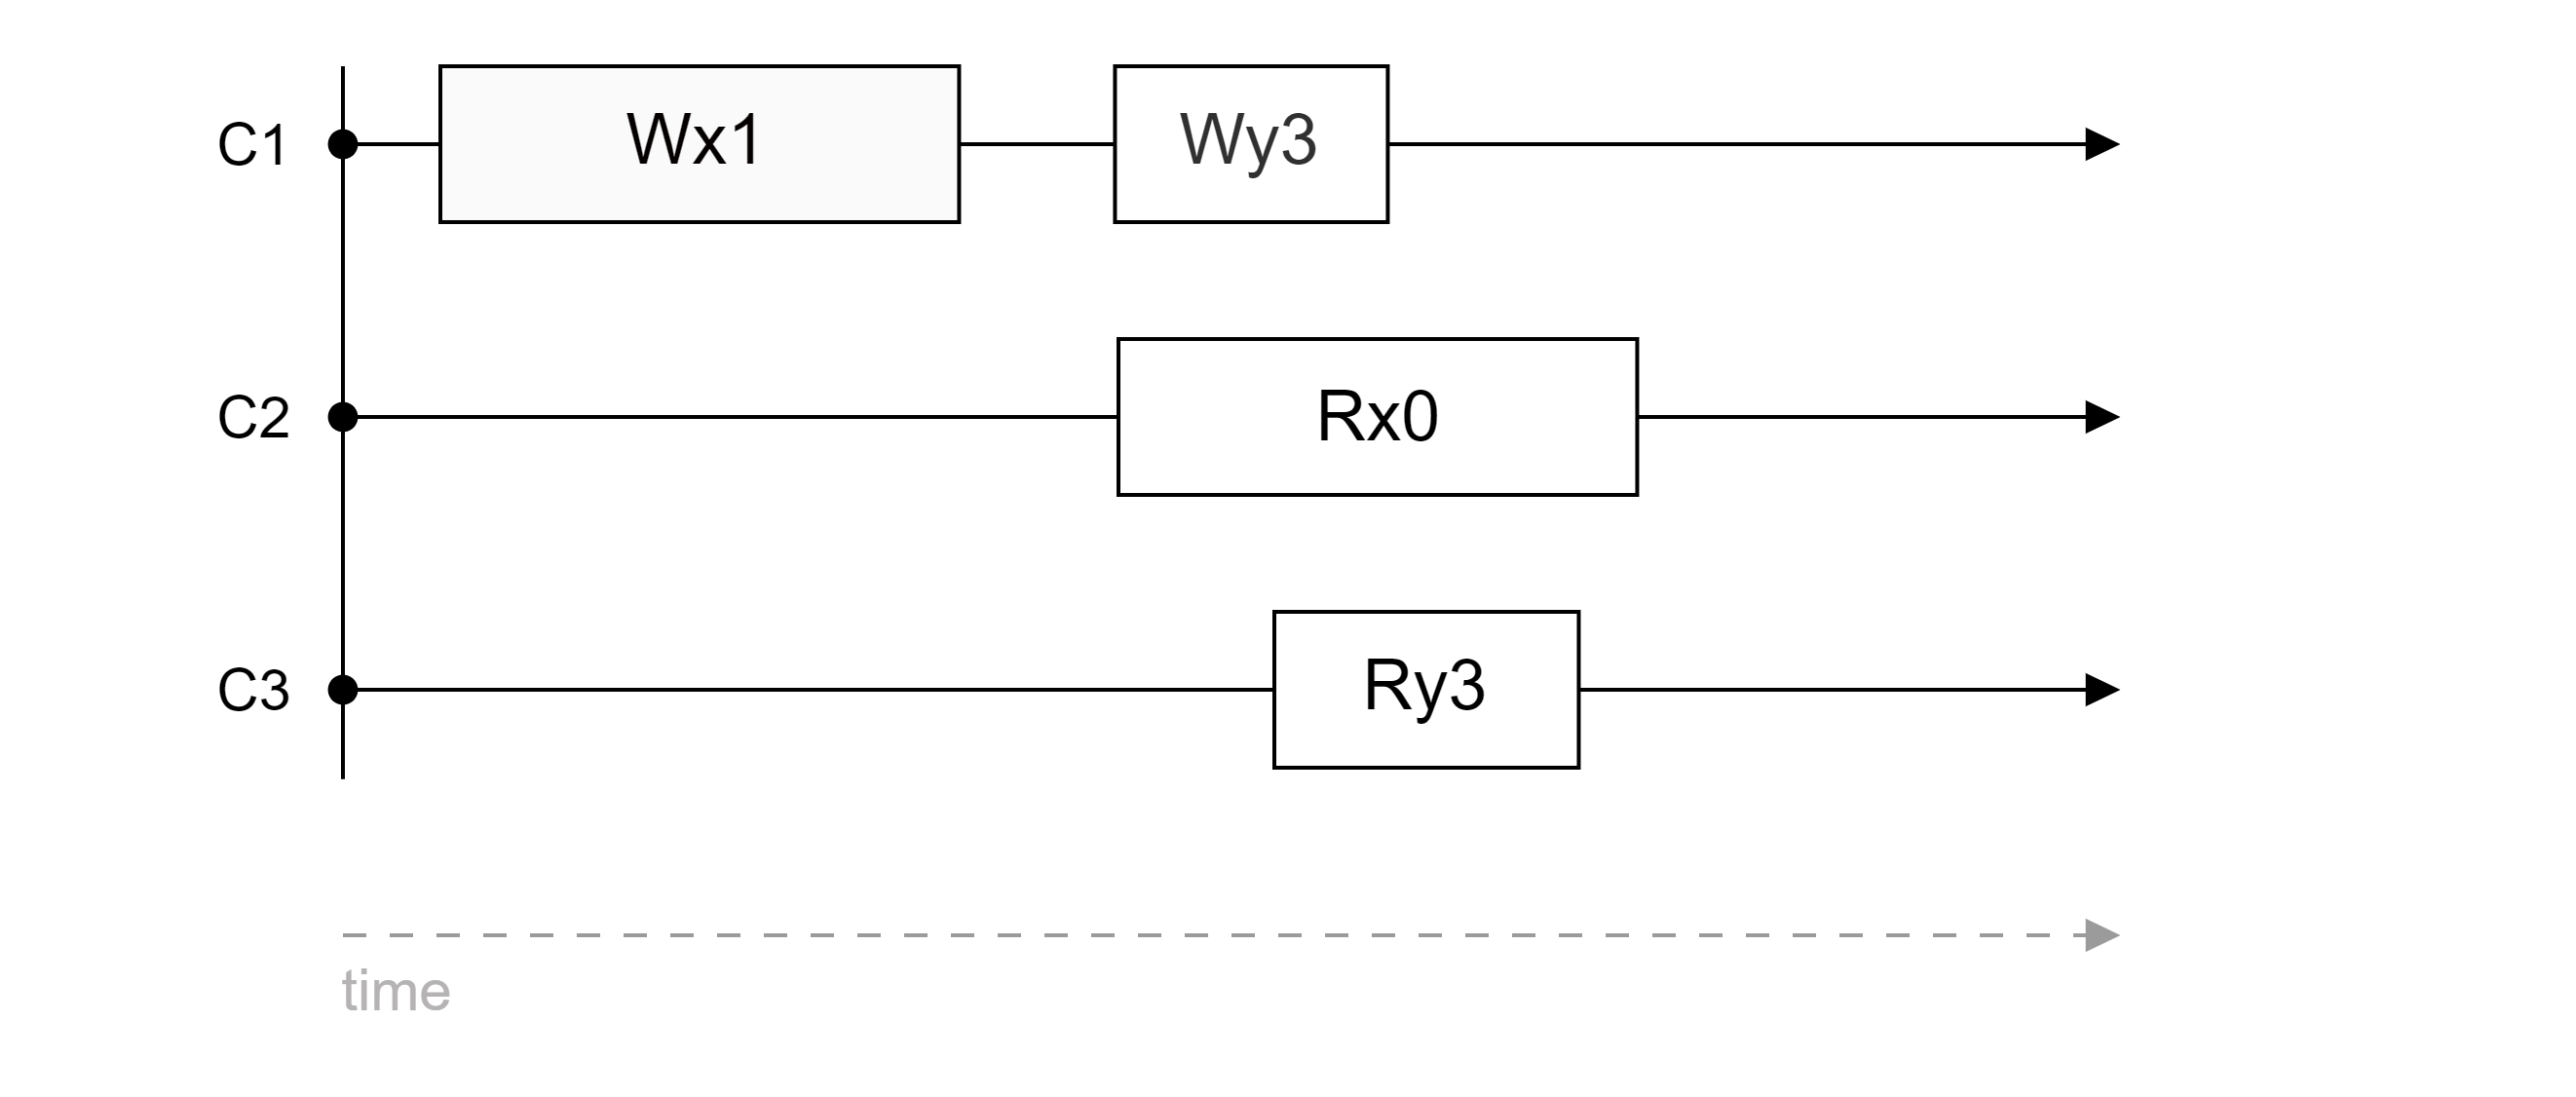
\includegraphics[width=\textwidth]{Sections/consist/lin1.png}
    \caption{A distributed system with client C1, C2, and C3 interactions. Where $Wx1$ reads, ``Write 1 to x'' and $Rx0$ reads, ``0 read from x.'' This 
    system is not linearizable because the read $Rx0$ should have returned 1, in respect to real-time.}
\end{figure}

\begin{figure}[h]
    \centering
    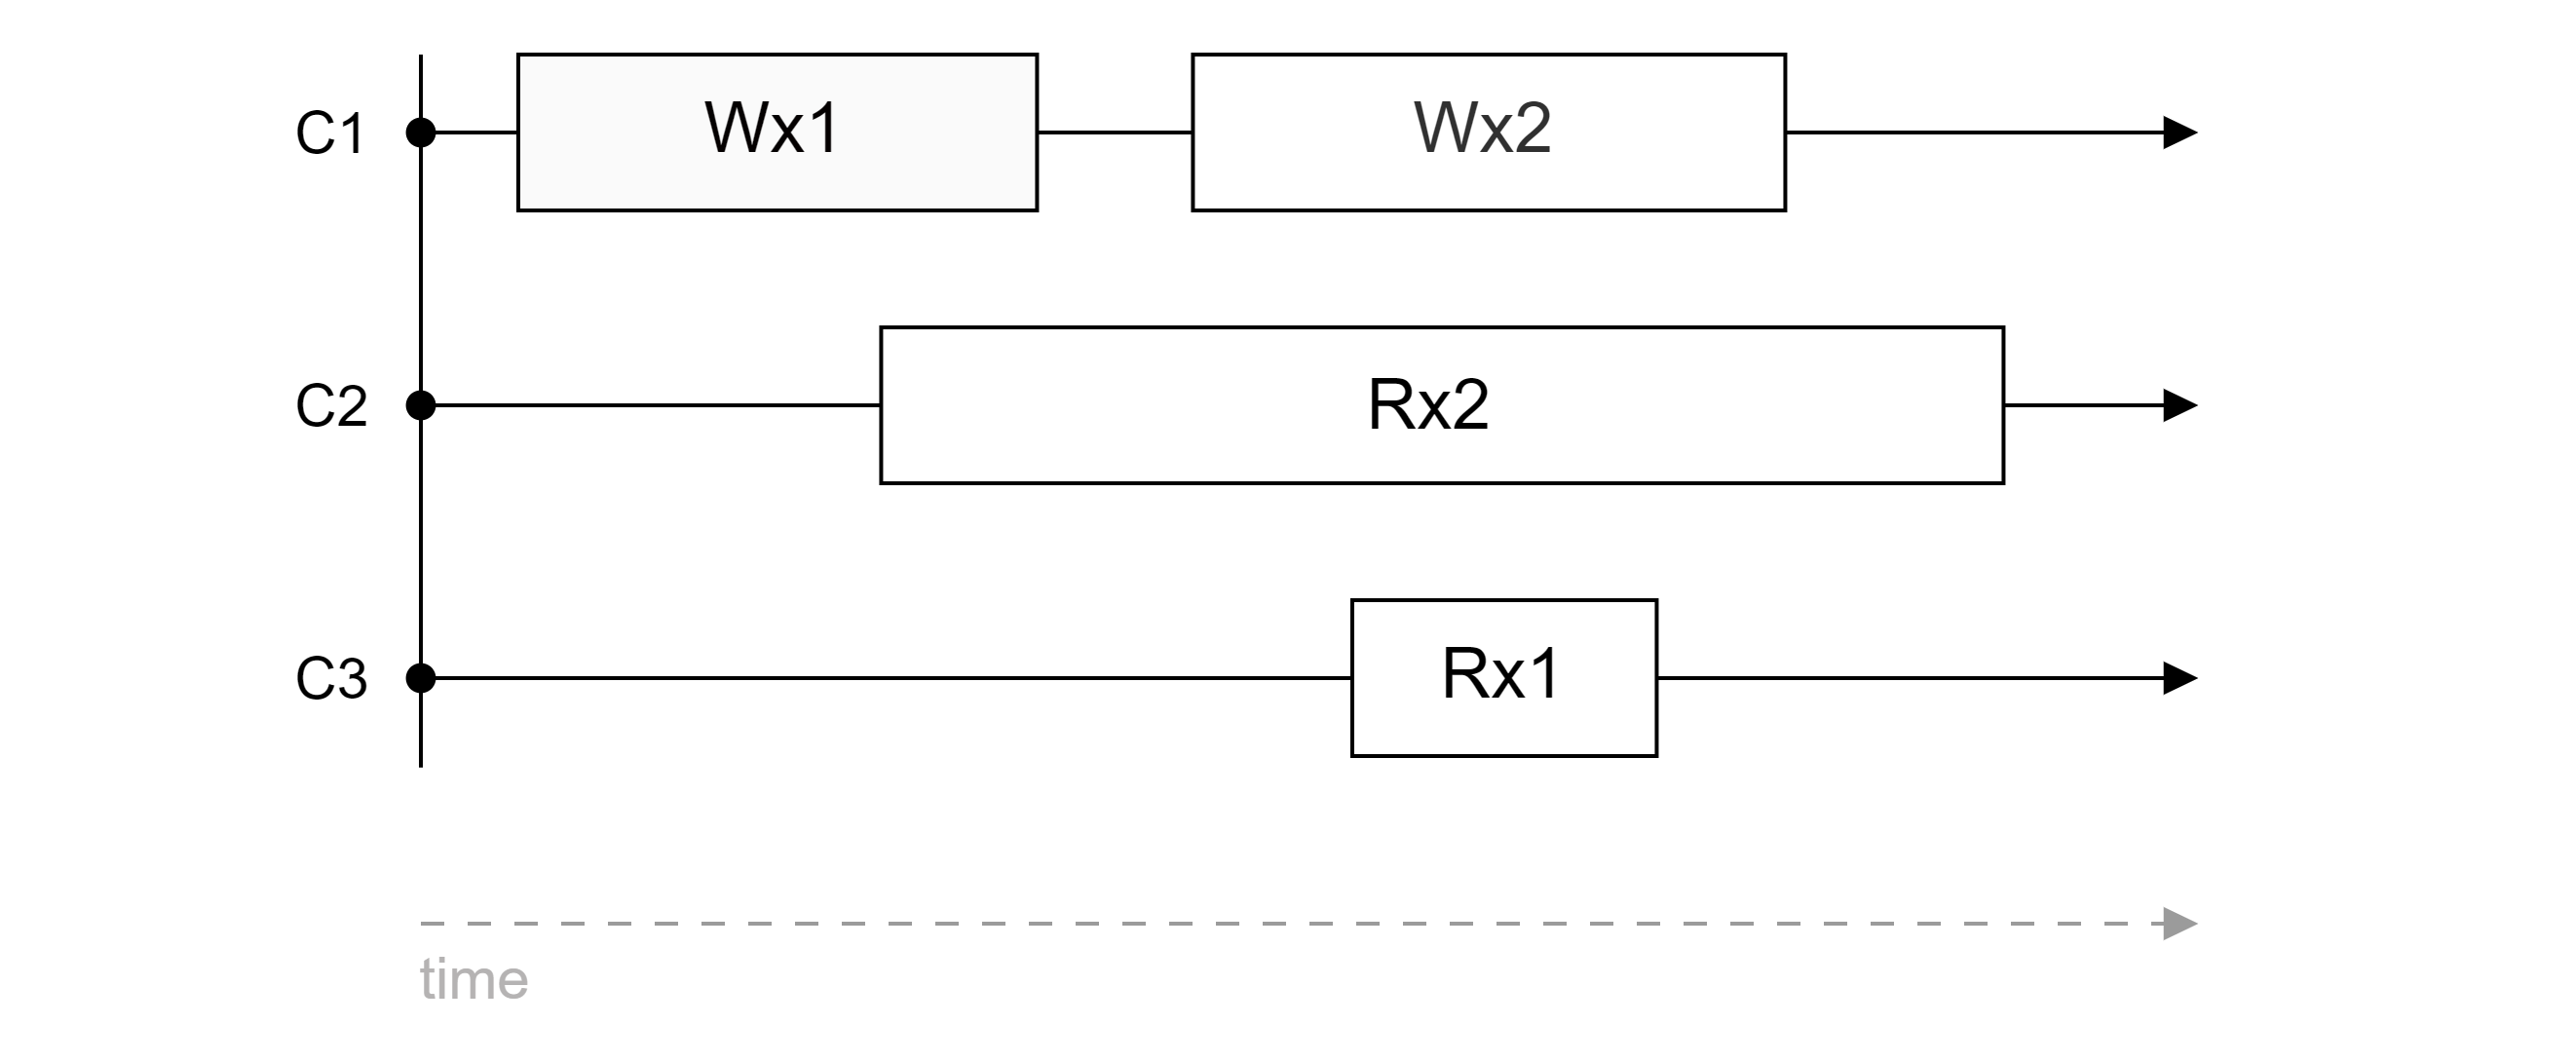
\includegraphics[width=\textwidth]{Sections/consist/lin2.png}
    \caption{A distributed system with client C1, C2, and C3 interactions. Where $Wx1$ reads, ``Write 1 to x'' and $Rx1$ reads, ``1 read from x.'' This
    system is linearizable. This is because each box represents a period of time when the action could take place. Therefore, Wx1 and Rx1 can happen, while still having enough time for Wx2 and Rx2 to occur.}
    \label{fig:my_label}
\end{figure}

\noindent
The \textbf{next page} includes an elaboration of the above.

\newpage 

\noindent
Here we elaborate on Figure (\ref{fig:my_label}):
\begin{figure}[h]
    \centering 
    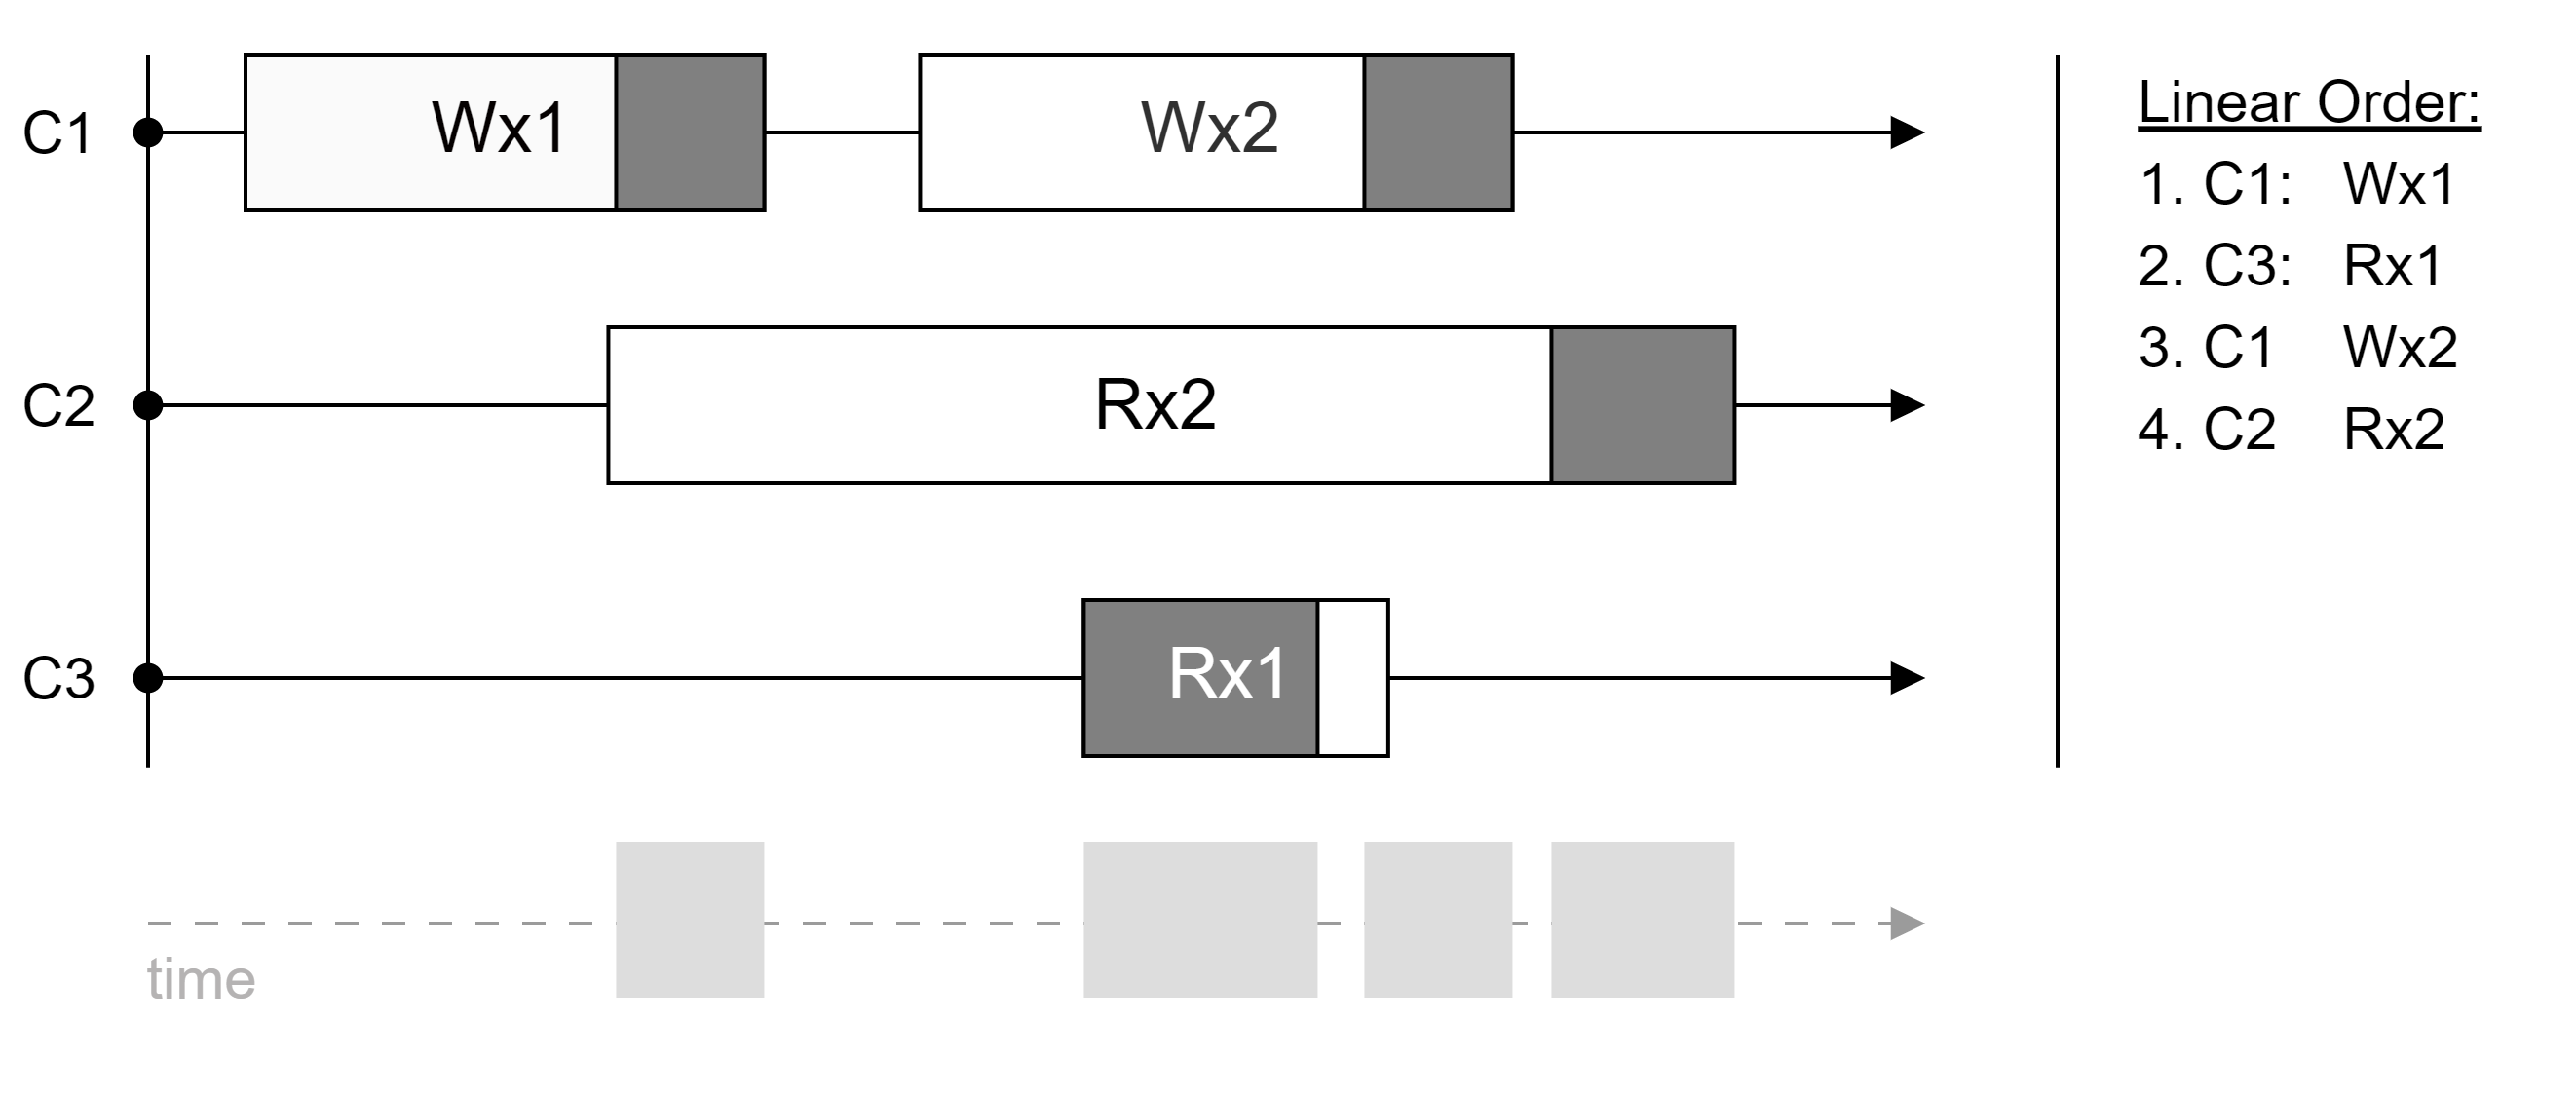
\includegraphics[width=\textwidth]{Sections/consist/lin3.png}
    \caption{The gray boxes represent a mutex on the shared data, $x$. Here we see the order of operations, Wx1, Rx1, Wx2, and Rx2, from which \textbf{no overlaps occur} and logically make sense.}
\end{figure}

\begin{figure}[h]
    \centering
    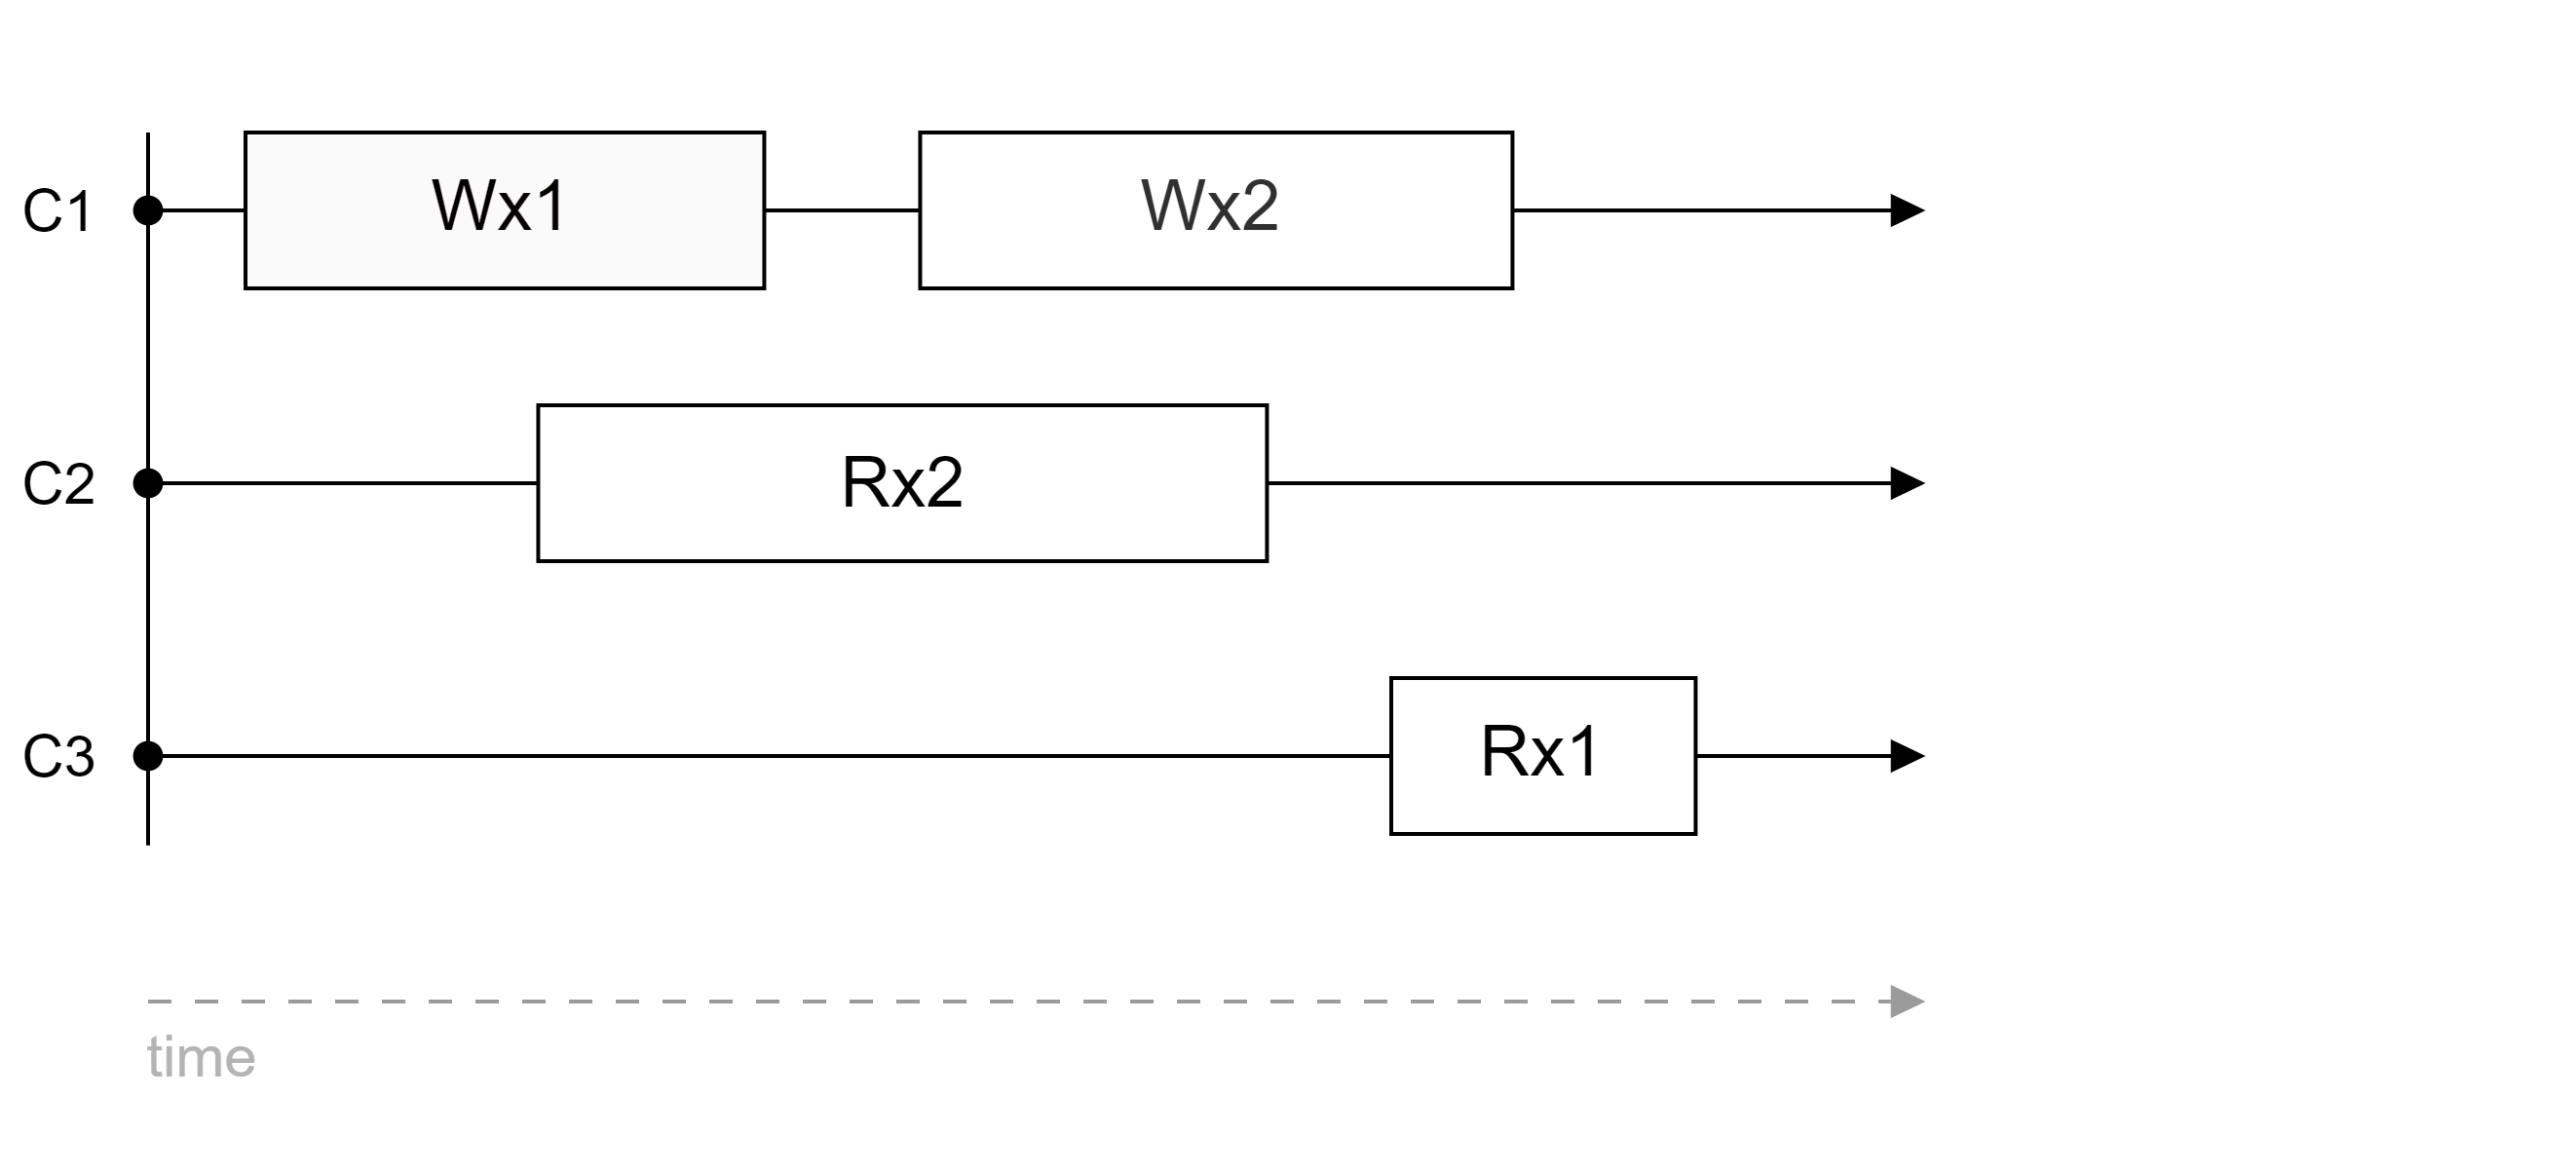
\includegraphics[width=\textwidth]{Sections/consist/lin4.png}
    \caption{A distributed system with client C1, C2, and C3 interactions. Where $Wx1$ reads, ``Write 1 to x'' and $Rx1$ reads, ``1 read from x.'' This
    system is not linearizable. The Rx1 is not possible as it's too far disjointed from Wx1 after being overwritten by Wx2. }
\end{figure}

\newpage

\noindent
We've talked about another replication method before that is also linearizable:
\begin{theo}[Chain Replication and Linearizability]
    
    Chain Replication is linearizable. The duration of a write operation extends until 
    the tail, from which an acknowledgment is sent. Reads also adhere to reading the last completed write,
    and is thus---a strong consistency model.
\end{theo}

\noindent
The next model is Sequential Consistency:
\begin{Def}[Sequential Consistency]
    
    \underline{\textbf{Weaker than Linearizability.}} All replicas execute all operations in \textbf{some} Global Total Order.
    Each client \textbf{observes the same order} once such order is agreed upon. Therefore a single machine may replicate the system
    if given such order. In particular:
    \begin{itemize}
        \item If a system process issues $A$ before $B$, then $A \rightarrow B$ in the Global Total Order.
        \item If $A$ and $B$ happen on different processes, there is no real-time ordering (concurrent).
    \end{itemize}
\end{Def}

\noindent
Consider the following examples and determine whether it is sequentially consistent:

\begin{figure}[h]
    \hspace{3em}
    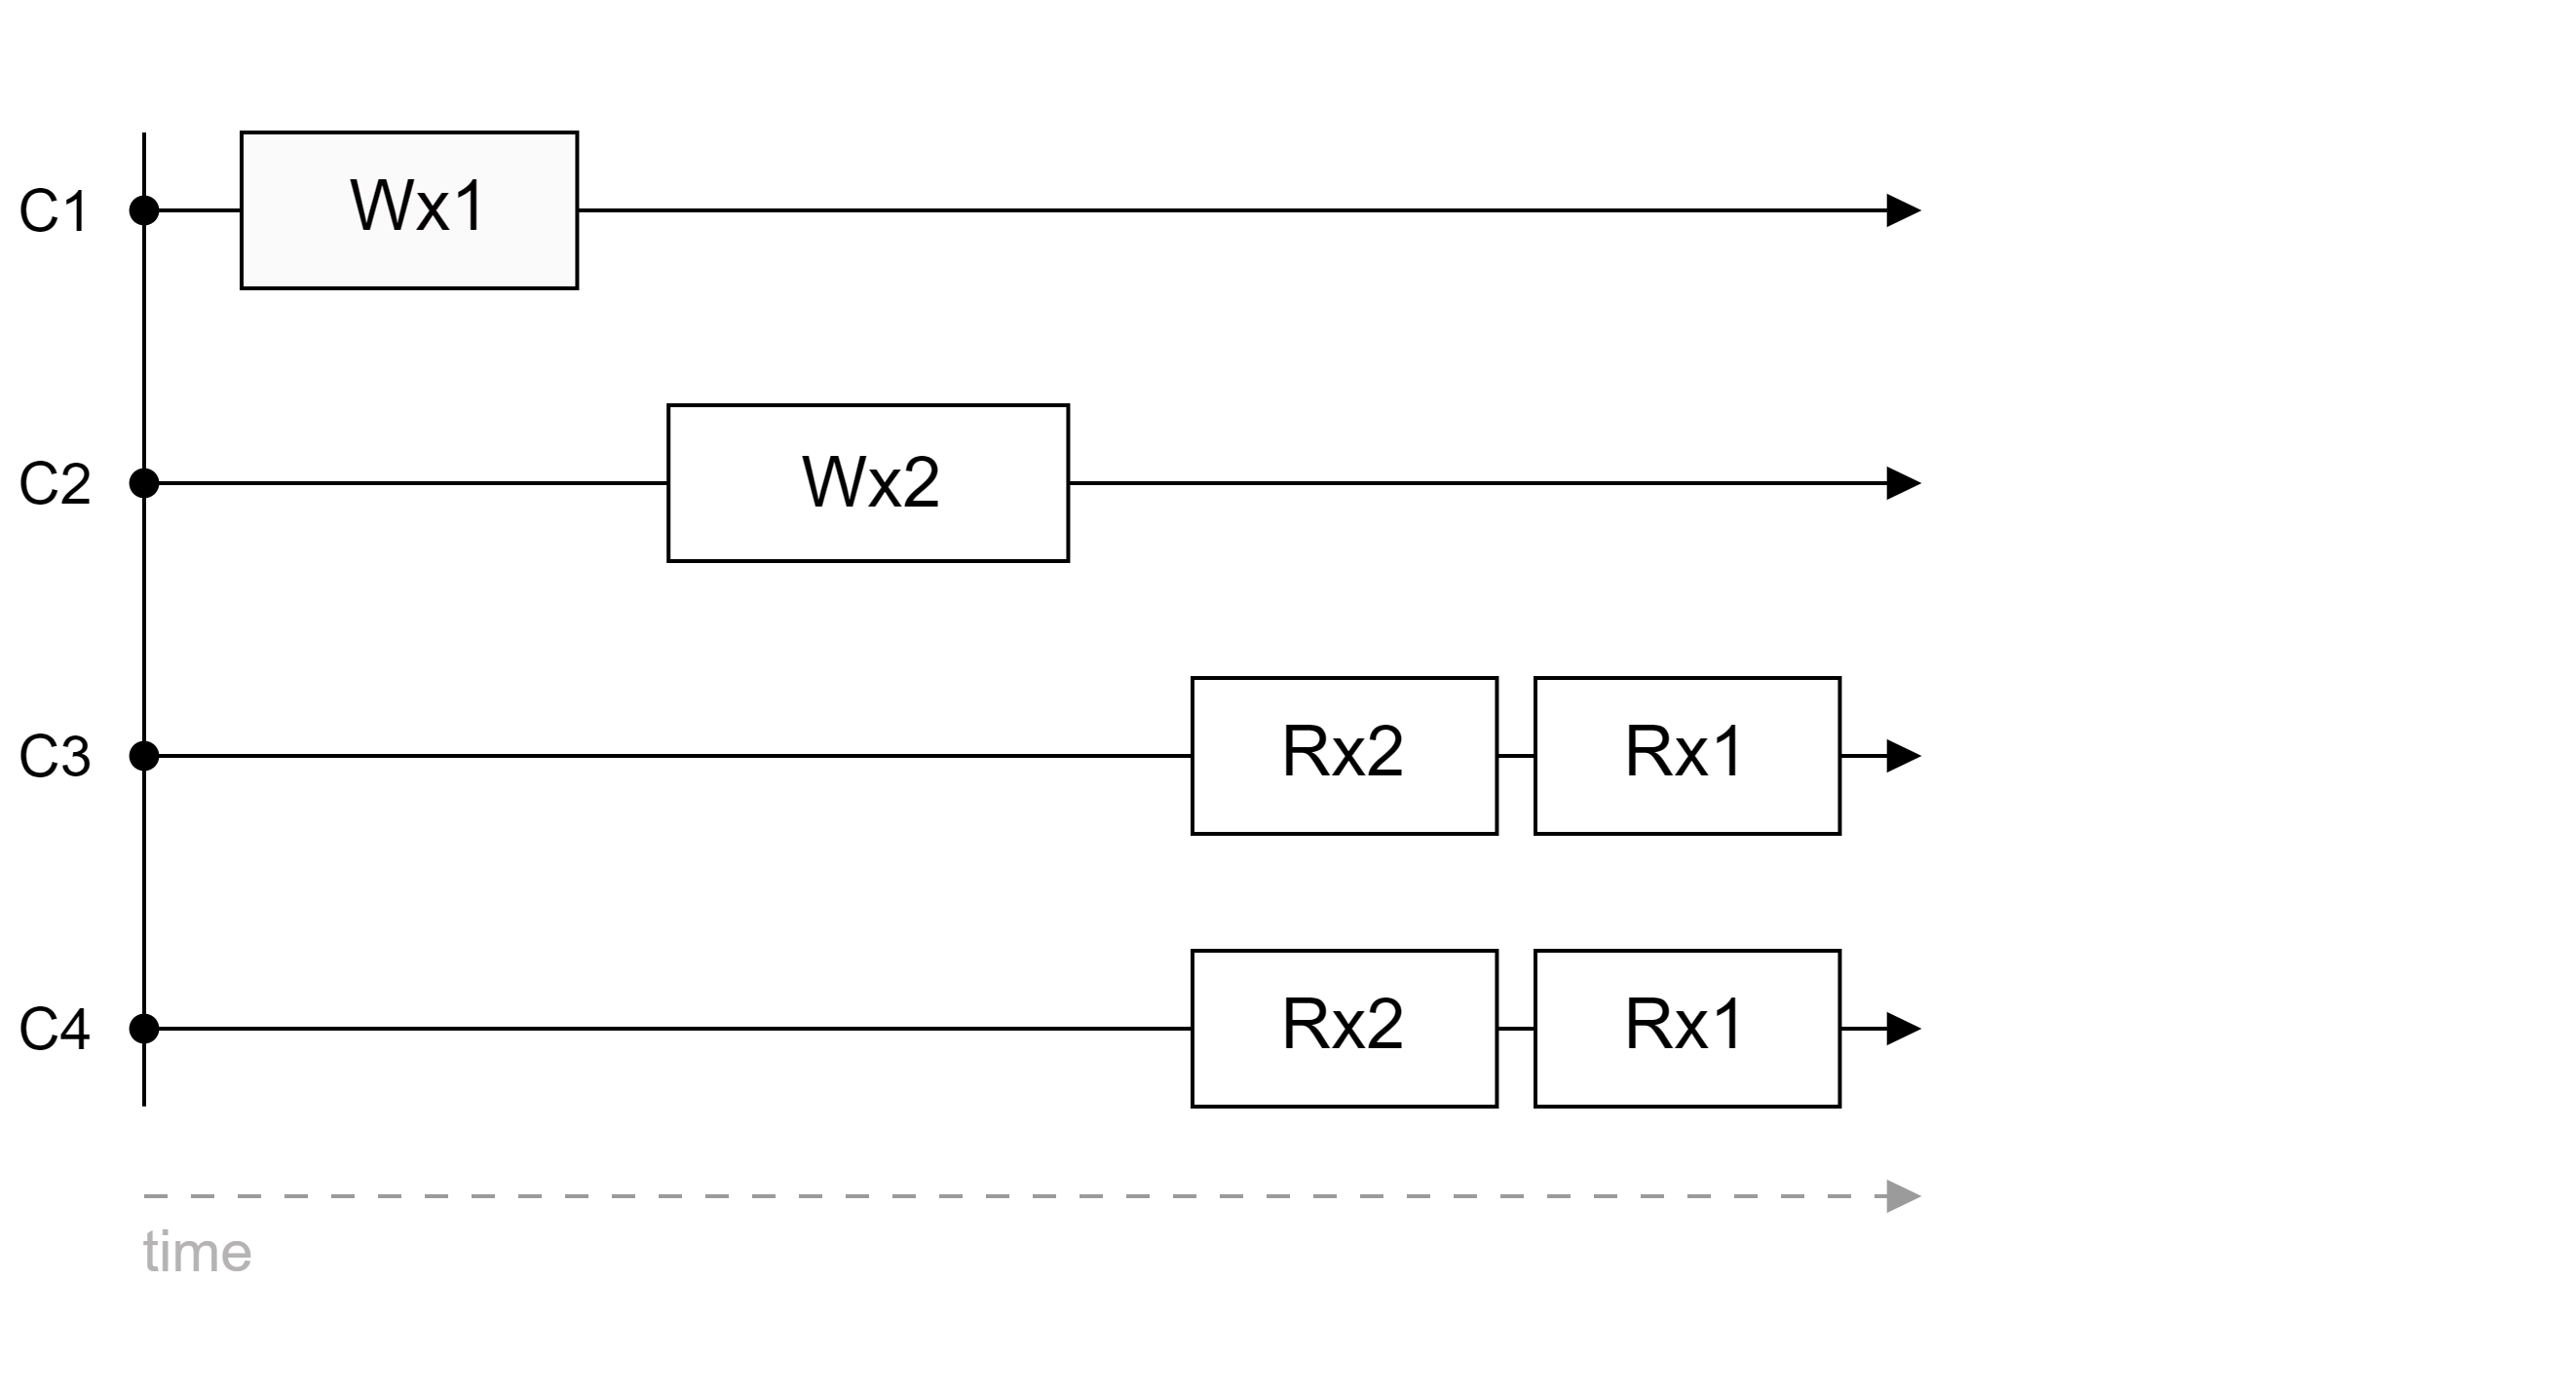
\includegraphics[width=.9\textwidth]{Sections/consist/seq1.png}
    \caption{A distributed system with client C1, C2, C3, C4 interactions. Where $Wx1$ reads, ``Write 1 to x'' and $Rx0$ reads, ``0 read from x.'' This 
    figure may or may not be sequentially consistent.}
\end{figure}

\noindent
\textbf{Next page} includes an elaboration of the above.

\newpage 

\noindent
We elaborate on the previous example:
\begin{figure}[h]
    \centering
    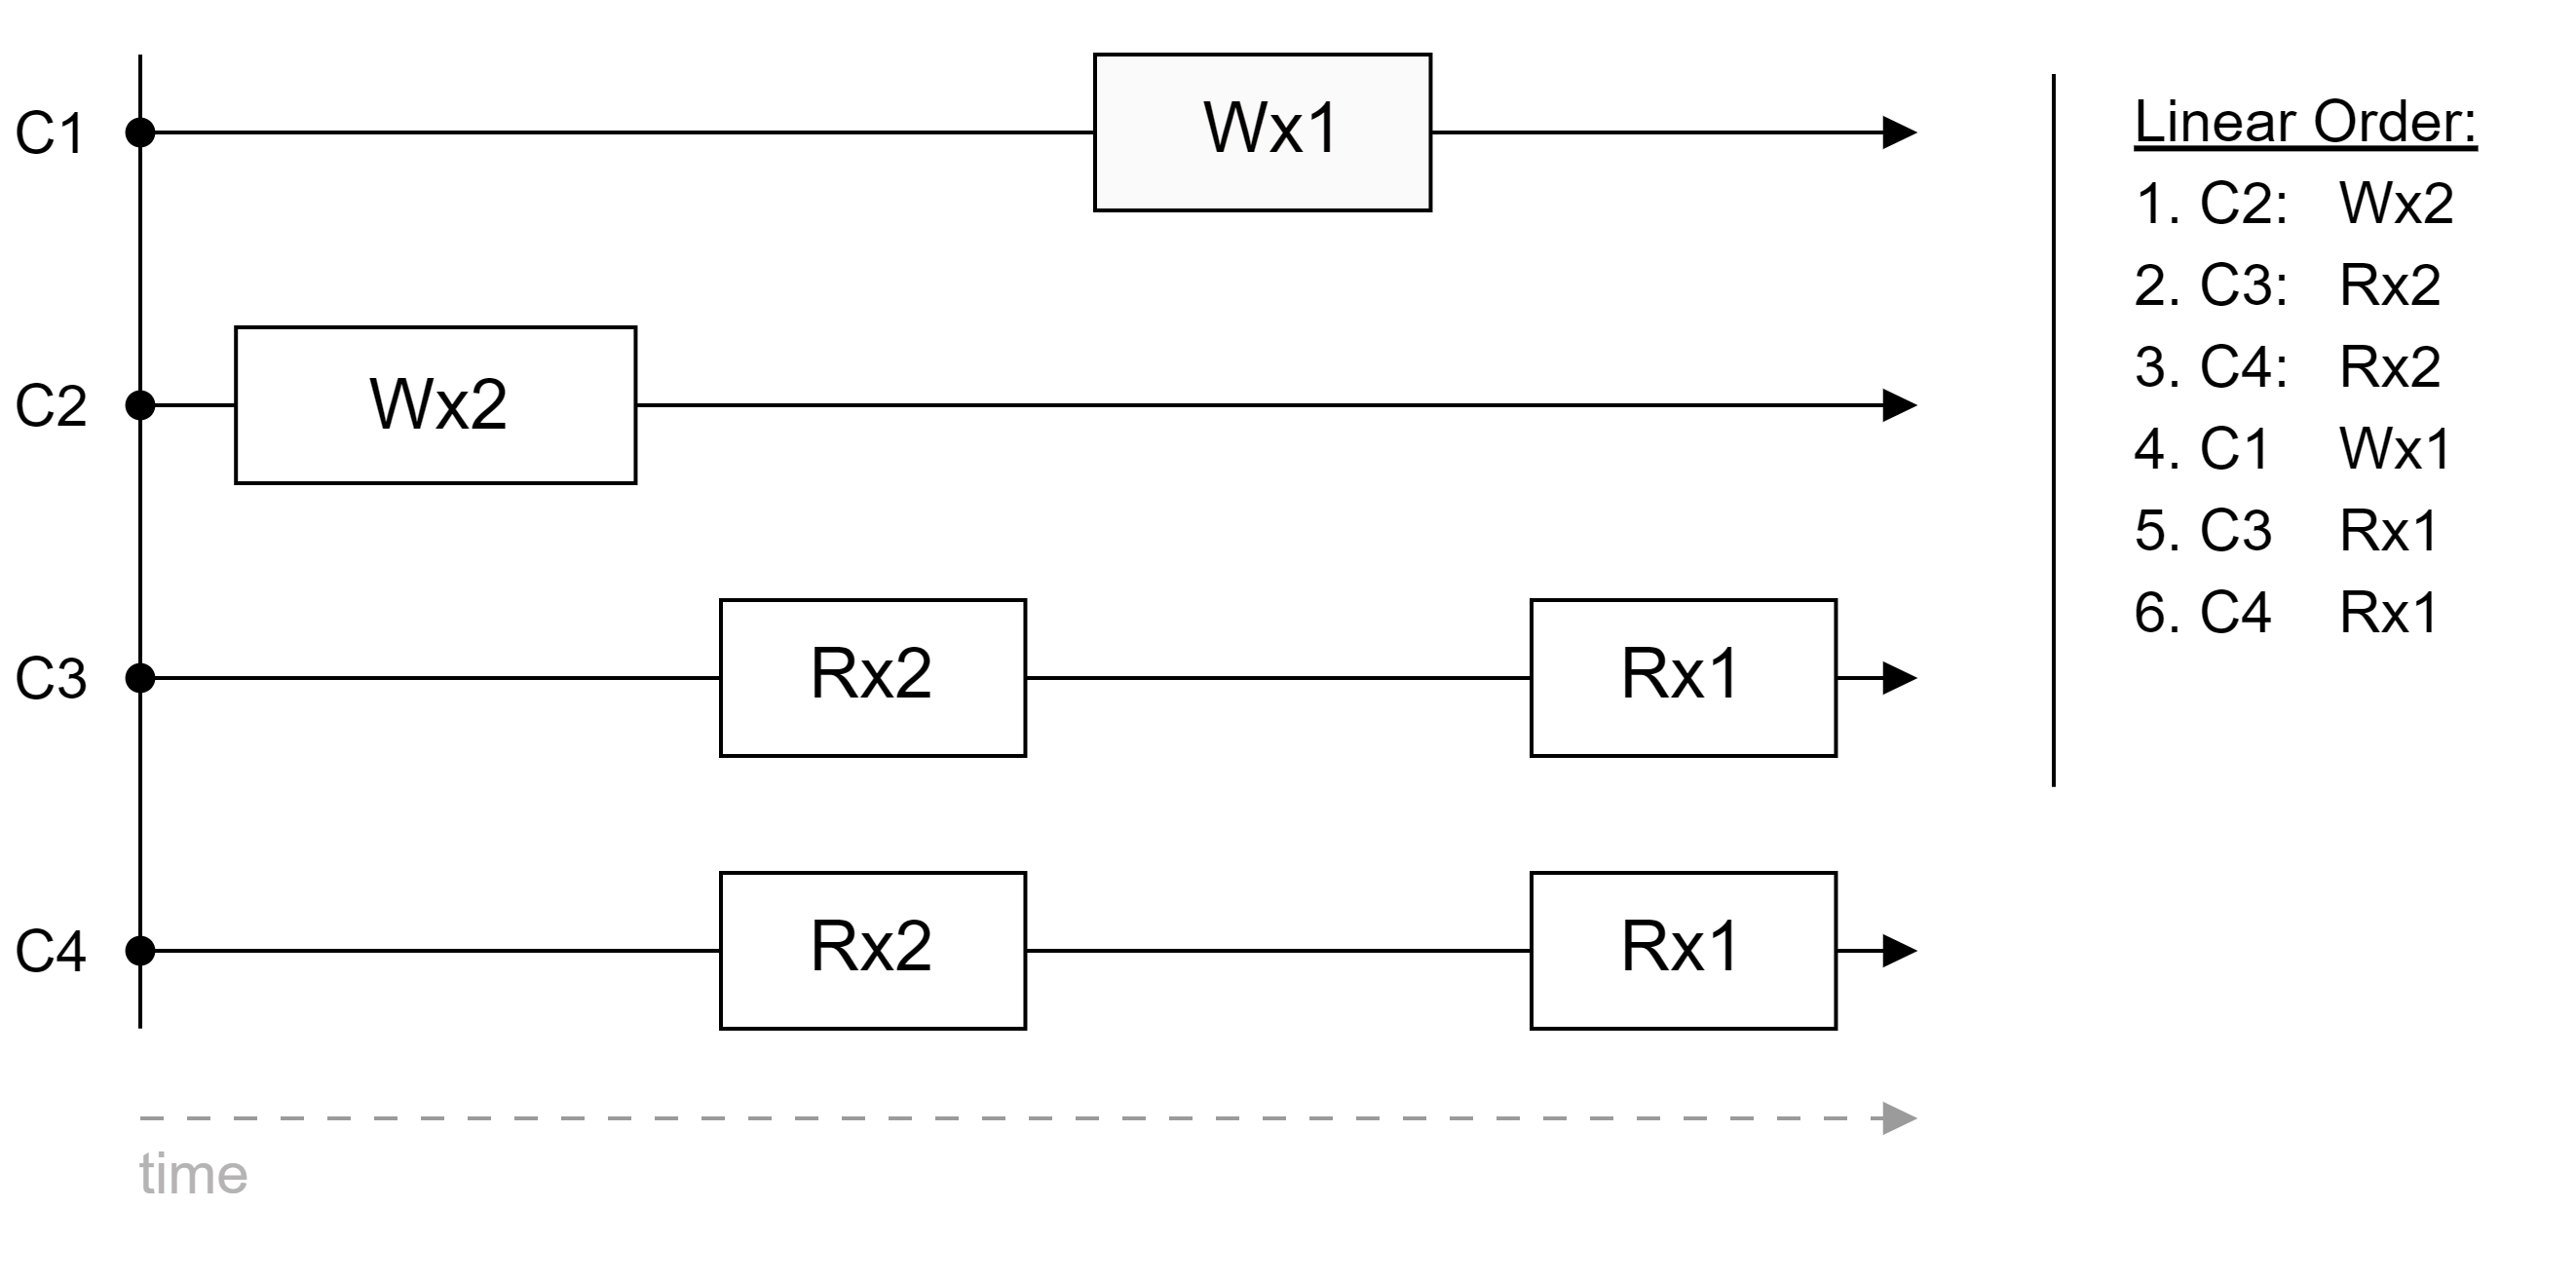
\includegraphics[width=.9\textwidth]{Sections/consist/seq2.png}
    \caption{A distributed system with client C1, C2, C3, C4 interactions. Where $Wx1$ reads, ``Write 1 to x'' and $Rx1$ reads, ``1 read from x.''. This 
    figure is sequentially consistent as there exists some Global Total Order that can be agreed upon. Here listed, Wx2, Rx2, Rx2, Wx1, Rx1, Rx1.}
\end{figure}

\noindent
And lastly, consider the following example:\\

\vspace{-1em}
\begin{figure}[ht!]
    \centering
    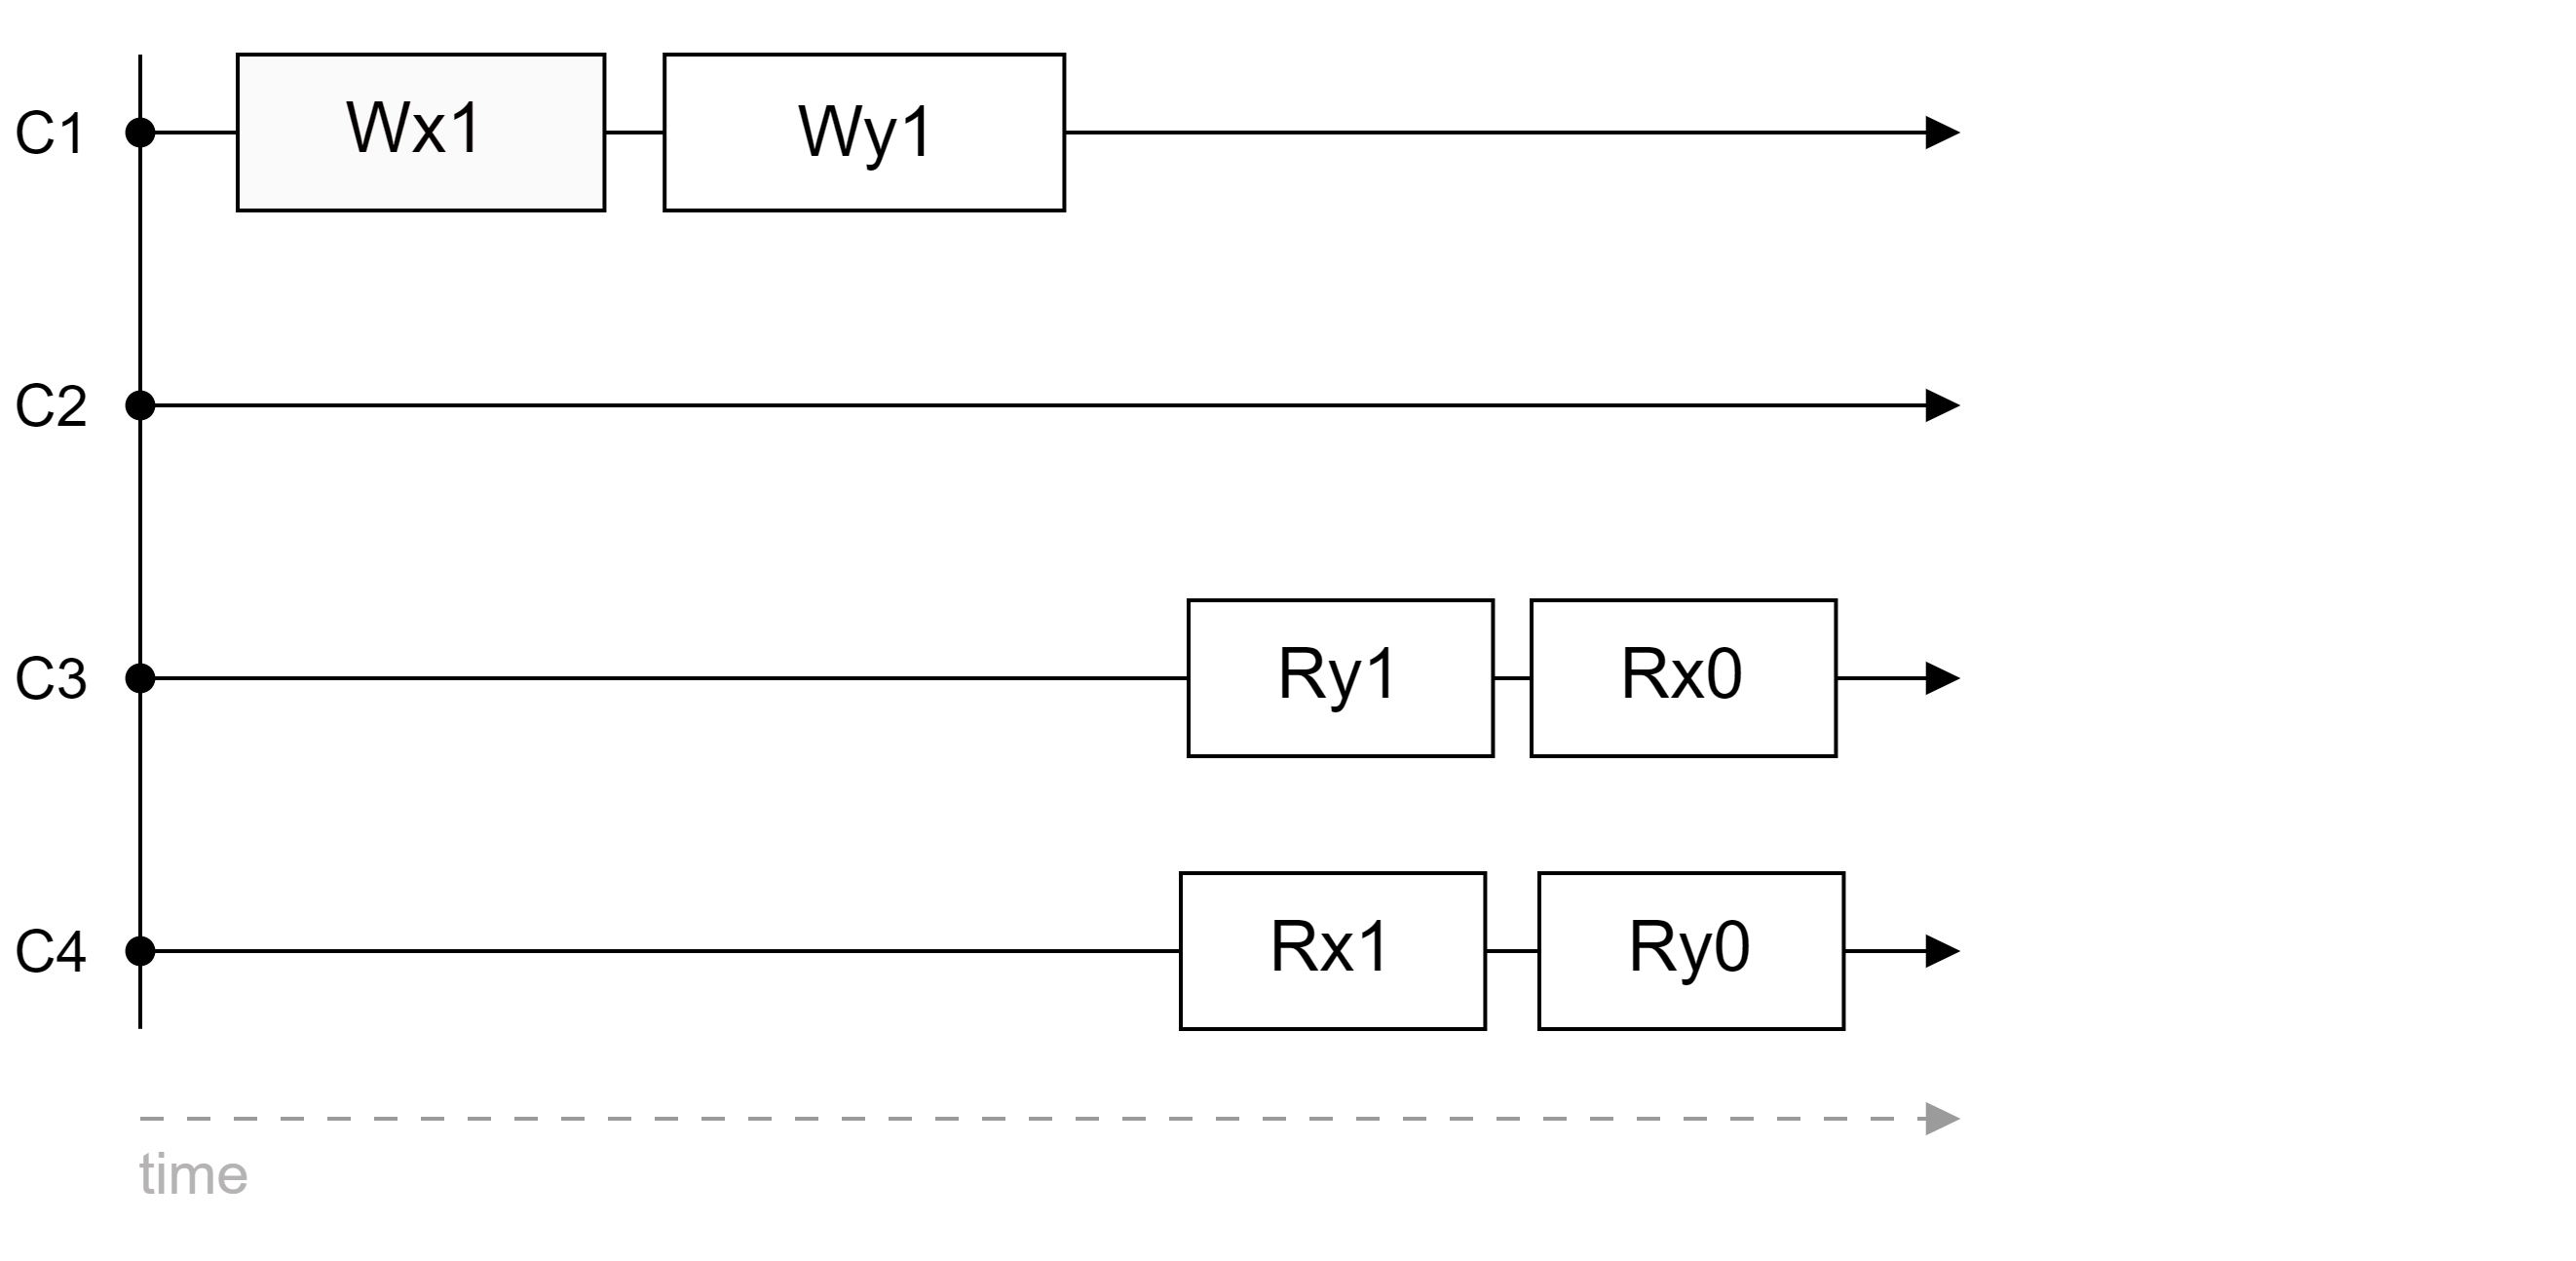
\includegraphics[width=.9\textwidth]{Sections/consist/seq3.png}
    \caption{A distributed system with client C1, C2, C3, C4 interactions. Where $Wx1$ reads, ``Write 1 to x'' and $Rx1$ reads, ``1 read from x.''. This 
    figure is not sequentially consistent as there is no Global Total Order that can be agreed upon. Here Rx0 cannot happen after Ry1 because 
    of the relation Wx1 $\rightarrow$ Wy1.}
    \label{fig:seq3}
\end{figure}



\newpage 

\noindent
Consider the following theorem:
\begin{theo}[Linearizability vs Sequential Consistency]
    
    If a system is linearizable, it is also sequentially consistent. As,  adhering to real-time order naturally satisfies sequential consistency.
    \textbf{However}, the reverse is not true. In particular:
    \begin{itemize}
        \item \textbf{Linearizability:} Relies on real-time.
        \item \textbf{Sequential Consistency:} Relies on program order.
    \end{itemize}
\end{theo}

\subsection{Handling Shared Data via Mutex: Release \& Lazy-release Consistency}

\noindent
Consider the following \textbf{Weak} methods of handling shared data:
\begin{Def}[Release Consistency vs. Lazy-release Consistency]
    
    These methods require explicit use of locks to propagate updates:\\
    \textbf{Release Consistency:} Push updates to all nodes after releasing the lock.\\
    \textbf{Lazy-release Consistency:} Push updates to all nodes after the lock is acquired.
    \textit{Though this may provide less stress to the system, if the client does not lock data, it may become stale (weak consistency).
    Alternatively, if the client locks all data (strong consistency) though it may be costly. }\underline{\textbf{These both are weak consistency models.}}
\end{Def}

\noindent
Determine whether the following system is release or lazy-release consistent:

\begin{figure}[h]
    \centering
    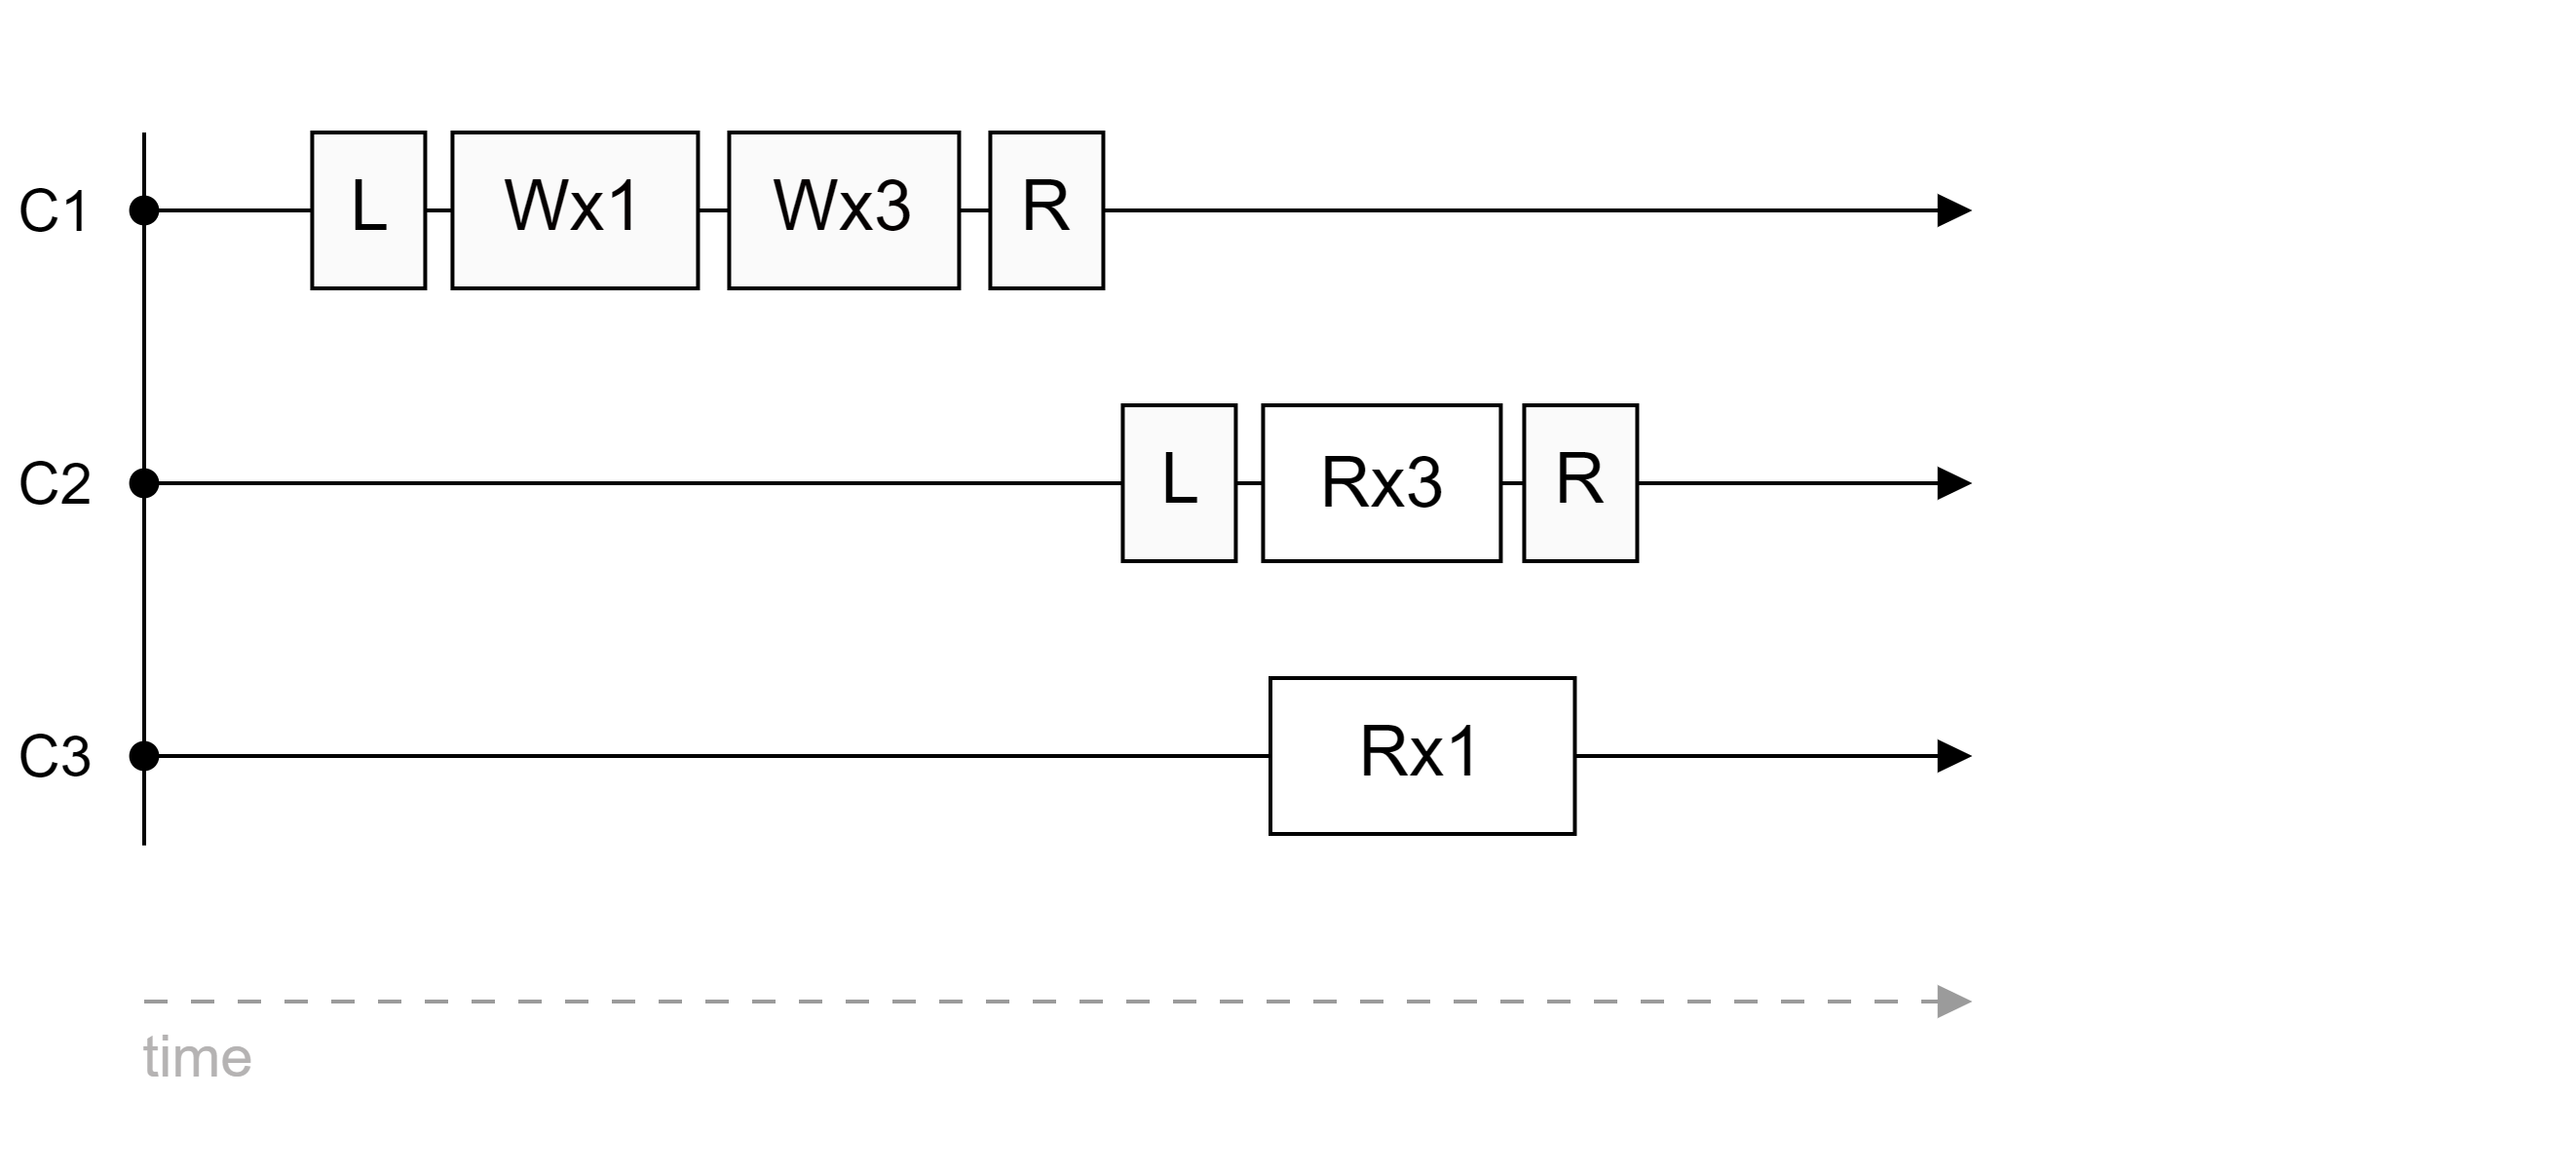
\includegraphics[width=.9\textwidth]{Sections/consist/rel.png}
    \caption{A distributed system with client C1, C2, and C3 interactions. Where $Wx1$ reads, ``Write 1 to x'' and $Rx1$ reads, ``1 read from x.'' This 
    is Lazy-release consistent, as C3's read of $x$ wasn't updated to 3 in absence of a lock.}
\end{figure}
\newpage 

\subsection{Weak Consistency Models: Causal \& Eventual Consistency}

We now discuss two weak consistency models, Causal Consistency and Eventual Consistency:

\begin{Def}[Causal Consistency]
    
    Weaker form of Sequential Consistency. That the Global Total Order of operations adhere logically to their causal dependencies.
    In particular: 
    \begin{itemize}
        \item If $A$ causes $B$, then $A \rightarrow B$ should be in the Global Total Order.
    \end{itemize}
\end{Def}

\noindent
For example, only one of these sentences makes causal sense:

\begin{center}
\begin{minipage}{0.30\textwidth}

    \noindent
(1)
\begin{enumerate}
    \item Alice: Lunch?
    \item Bob: Yes.
    \item Carl: No.
\end{enumerate}
\end{minipage}
\begin{minipage}{0.30\textwidth}
(2)
\begin{enumerate}
    \item Bob: Yes.
    \item Alice: Lunch?
    \item Carl: No.
\end{enumerate}
\end{minipage}
\begin{minipage}{0.30\textwidth}
    (3)
    \begin{enumerate}
        \item Alice: Lunch?
        \item Carl: No.
        \item Bob: Yes.
    \end{enumerate}
    \end{minipage}
\end{center}

\noindent
Here, statements (1) and (3) are causally consistent, as the responses are in order of the question. Take 
that same intuition for this next example and determine whether the below system is causally consistent:

\begin{figure}[h]
    \centering
    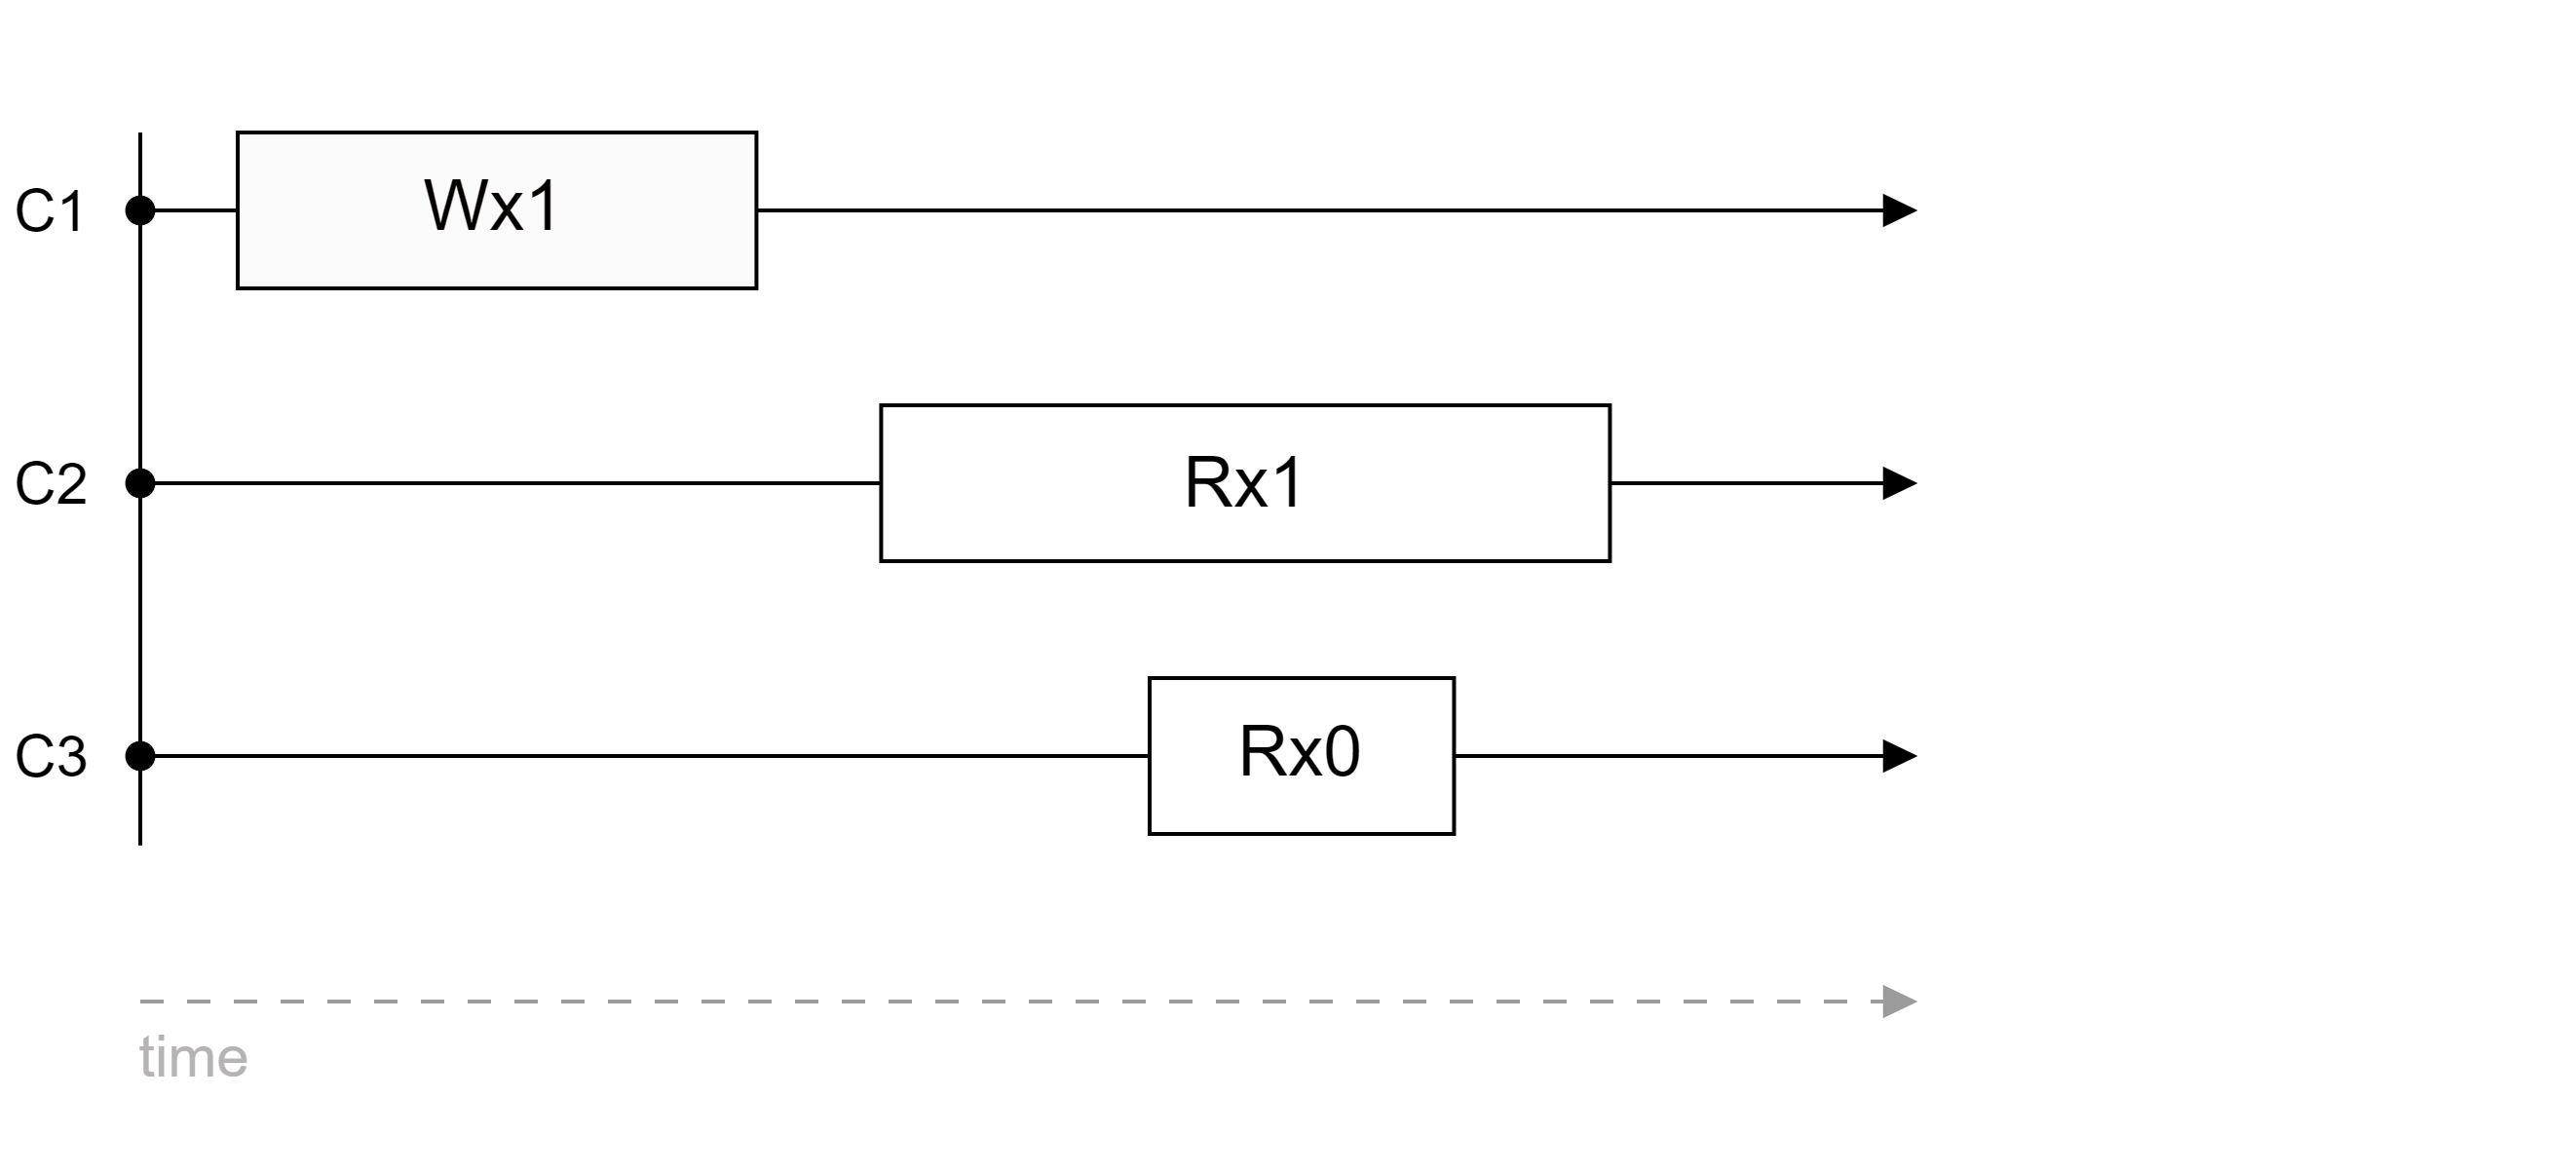
\includegraphics[width=.9\textwidth]{Sections/consist/cas1.png}
    \caption{A distributed system with client C1, C2, and C3 interactions. Where $Wx1$ reads, ``Write 1 to x'' and $Rx1$ reads, ``1 read from x.'' This 
    system is causally consistent as the Global Total Order of operations adhere to their causal dependencies. Here, Wx1 $\rightarrow$ Rx1, where Rx0 must come before Wx1.}
\end{figure}

\newpage 

\noindent
Consider the following example and determine whether it is causally consistent:
\begin{figure}[h] 
    \centering
    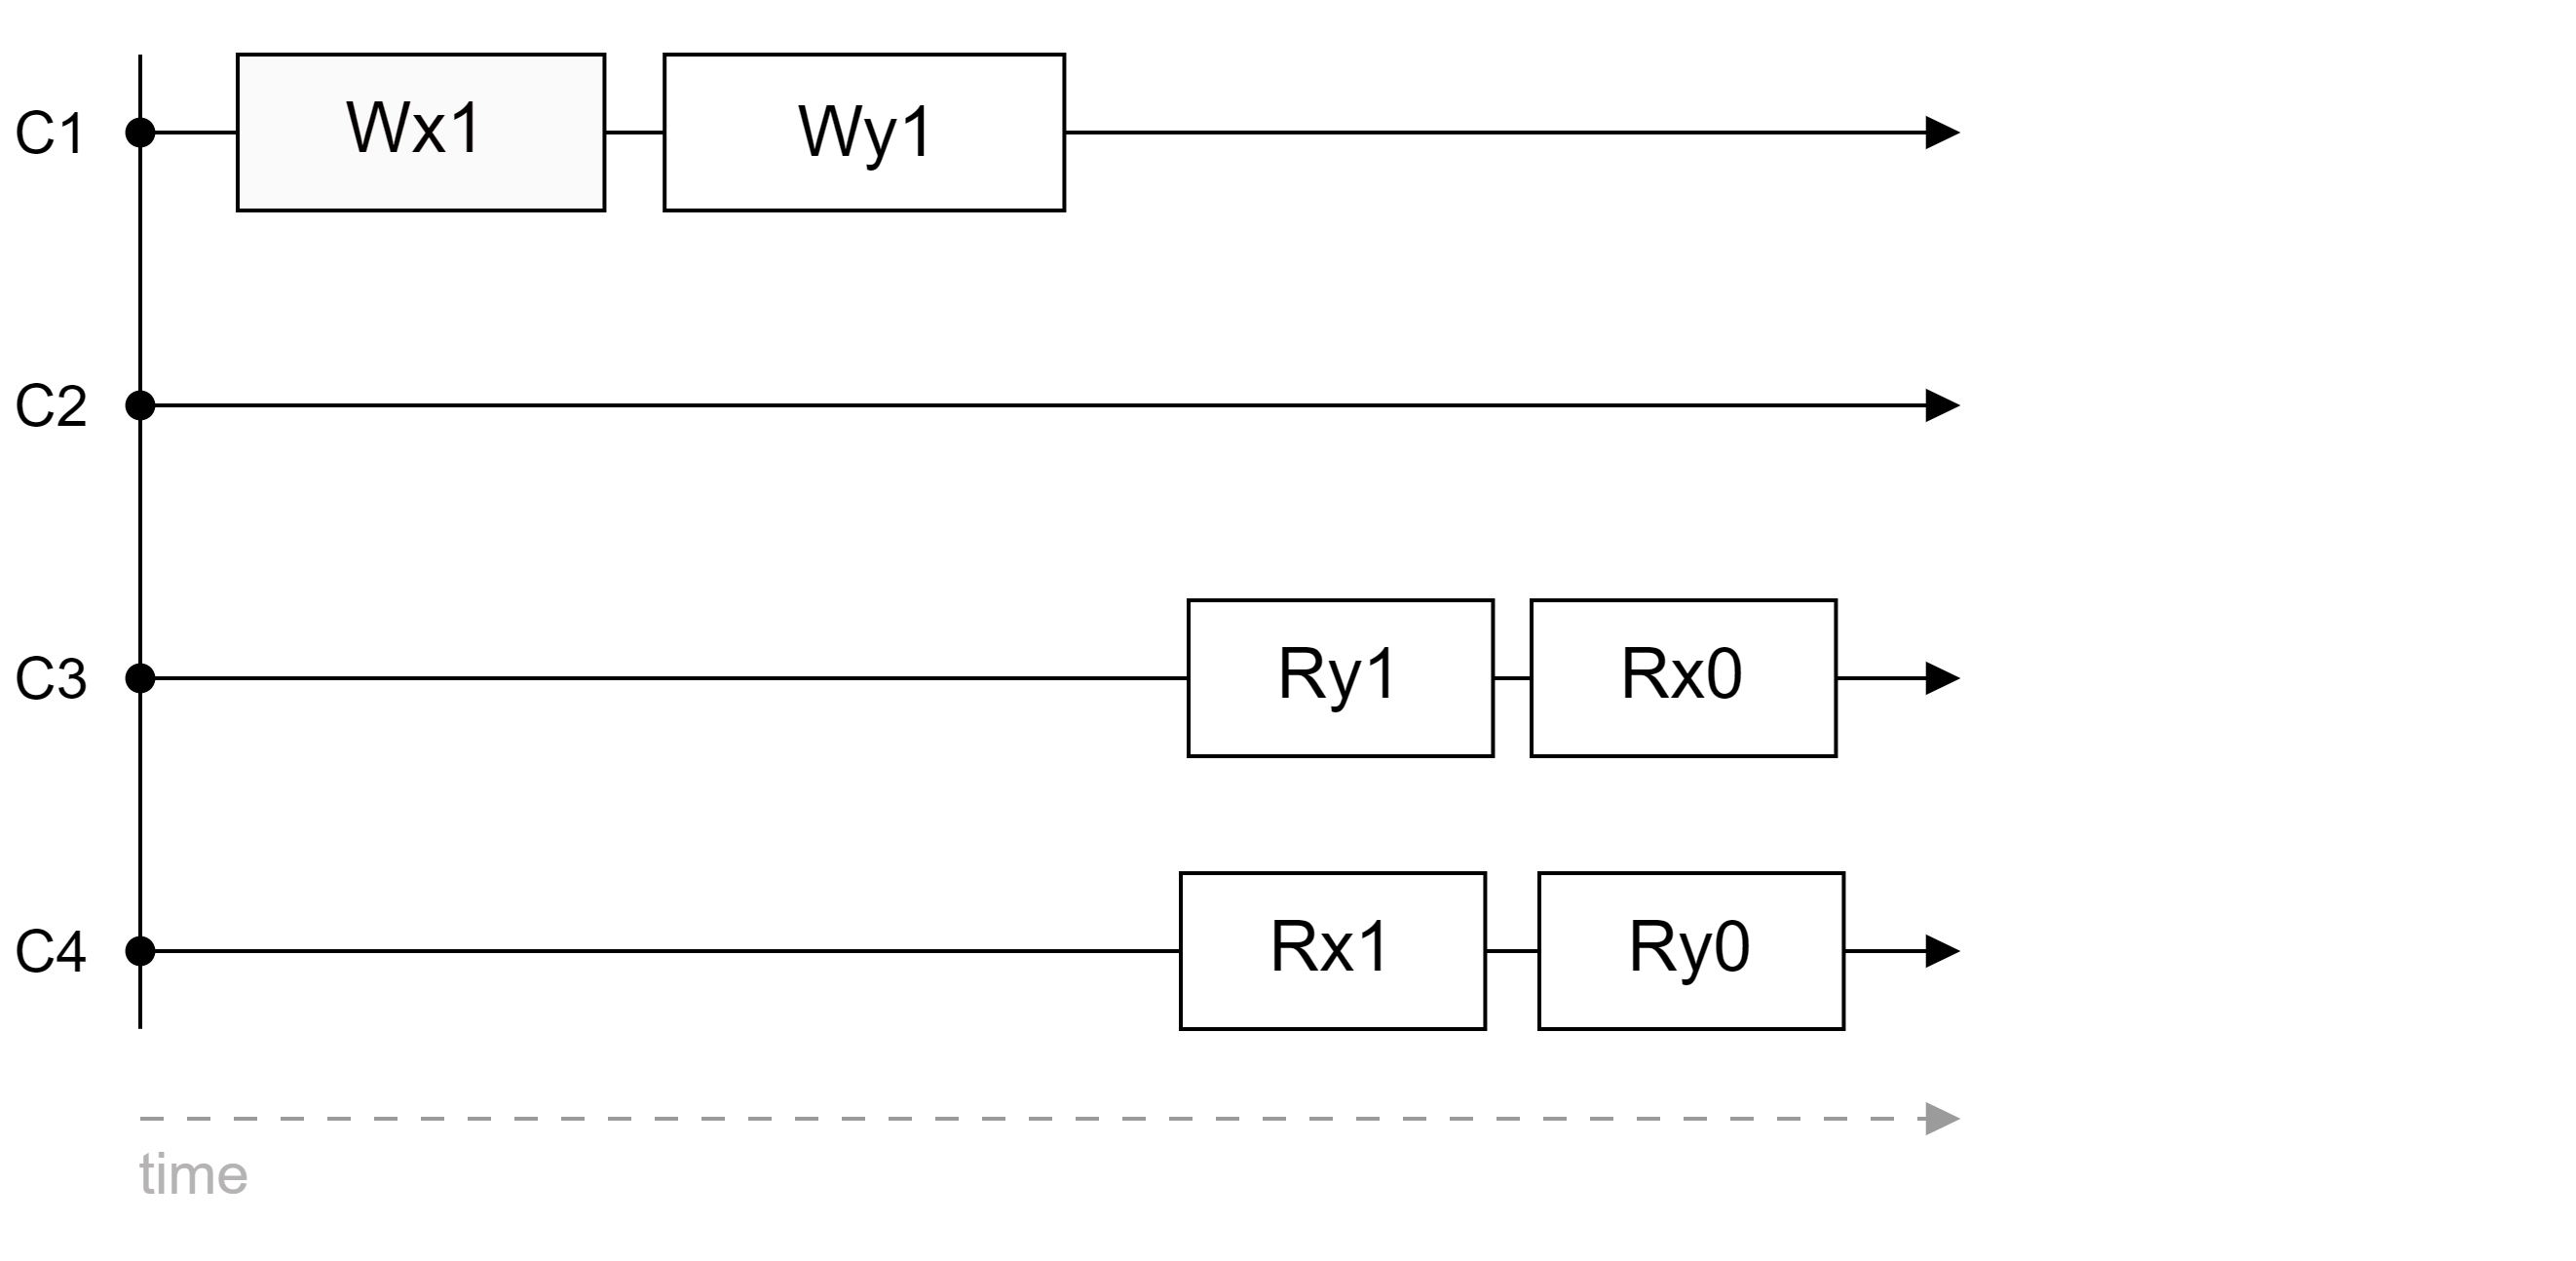
\includegraphics[width=.9\textwidth]{Sections/consist/seq3.png}
    \caption{This 
    System is not causally consistent for the same reasons as Figure (\ref{fig:seq3}) is not sequentially consistent.}
\end{figure}

\begin{Def}[Eventual Consistency]
    
    Weaker than Causal Consistency. Given there are no new writes, replicas will \textbf{eventually} agree on the same value 
    after some period of time.
\end{Def}

\begin{figure}[h]
    \centering
    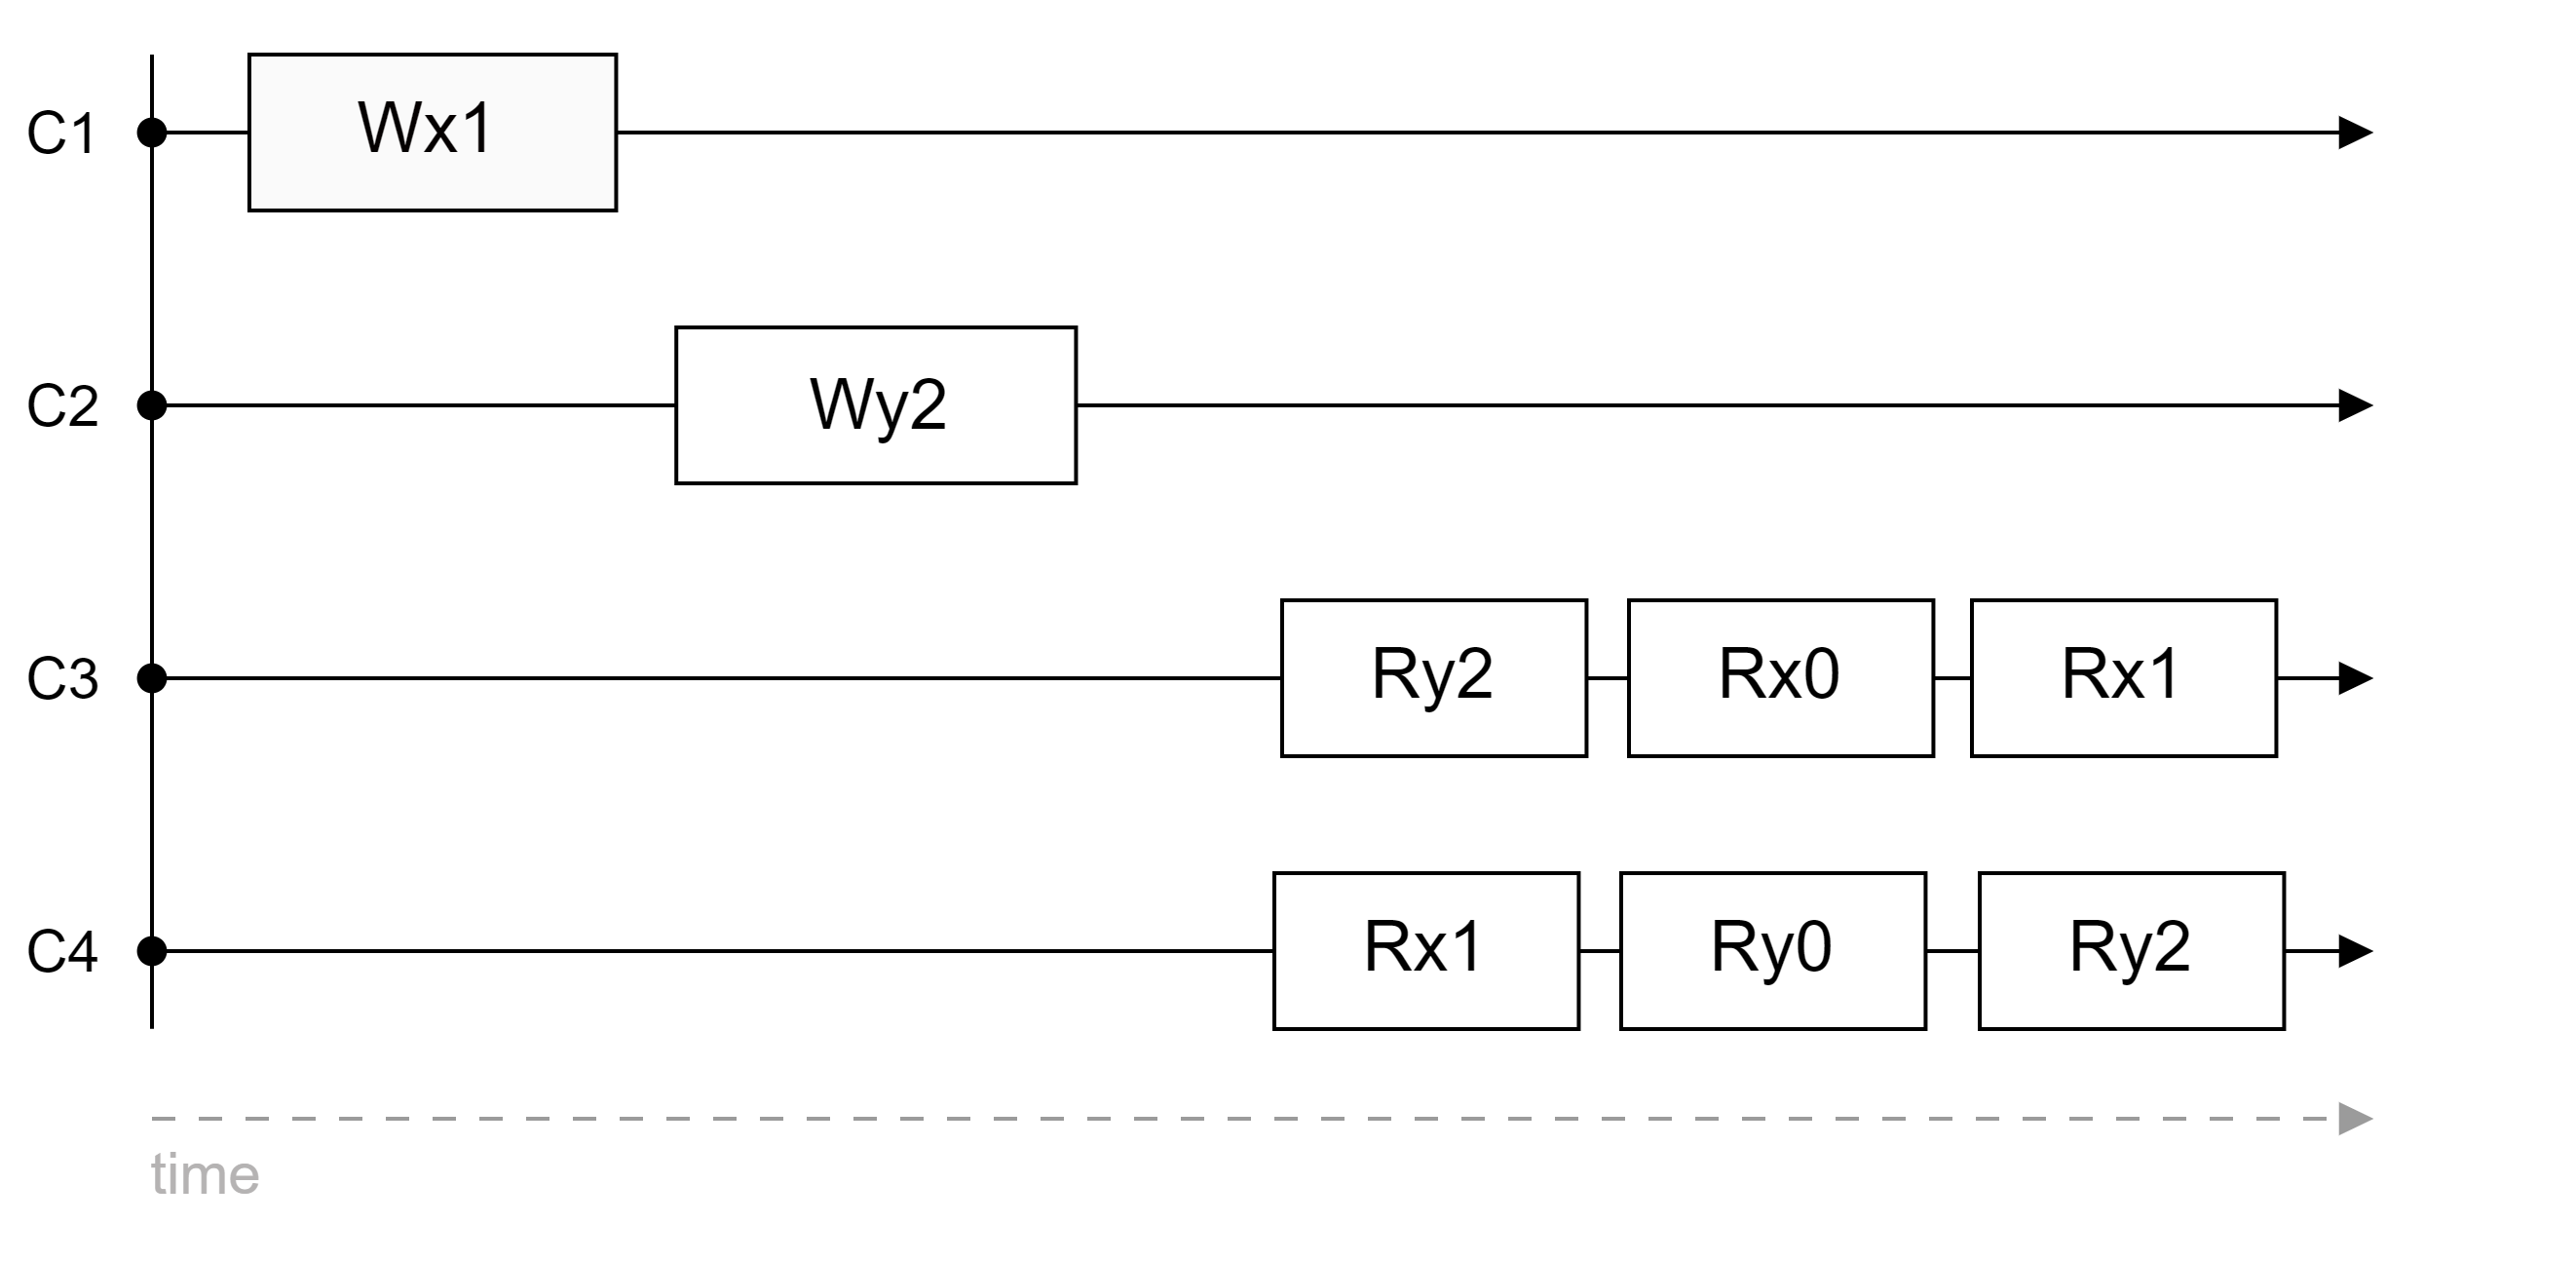
\includegraphics[width=.9\textwidth]{Sections/consist/event.png}
    \caption{This 
    system is eventually consistent as it eventually agrees on $x$ and $y$.}
\end{figure}

\newpage 

\noindent
Causal Consistency implies two properties:

\begin{theo}[Causal Consistency $\rightarrow$ FIFO \& RYW]

    Causal Consistency implies FIFO (First-In-First-Out) and RYW (Read-Your-Writes):
    \begin{itemize}
        \item \textbf{FIFO:} All writes are read in the order they were issued.
        \item \textbf{RYW:} If the client writes to $x$, then their next read of $x$ must return the value they just previously wrote.
    \end{itemize}
\end{theo}

\begin{figure}[h]
    \centering
    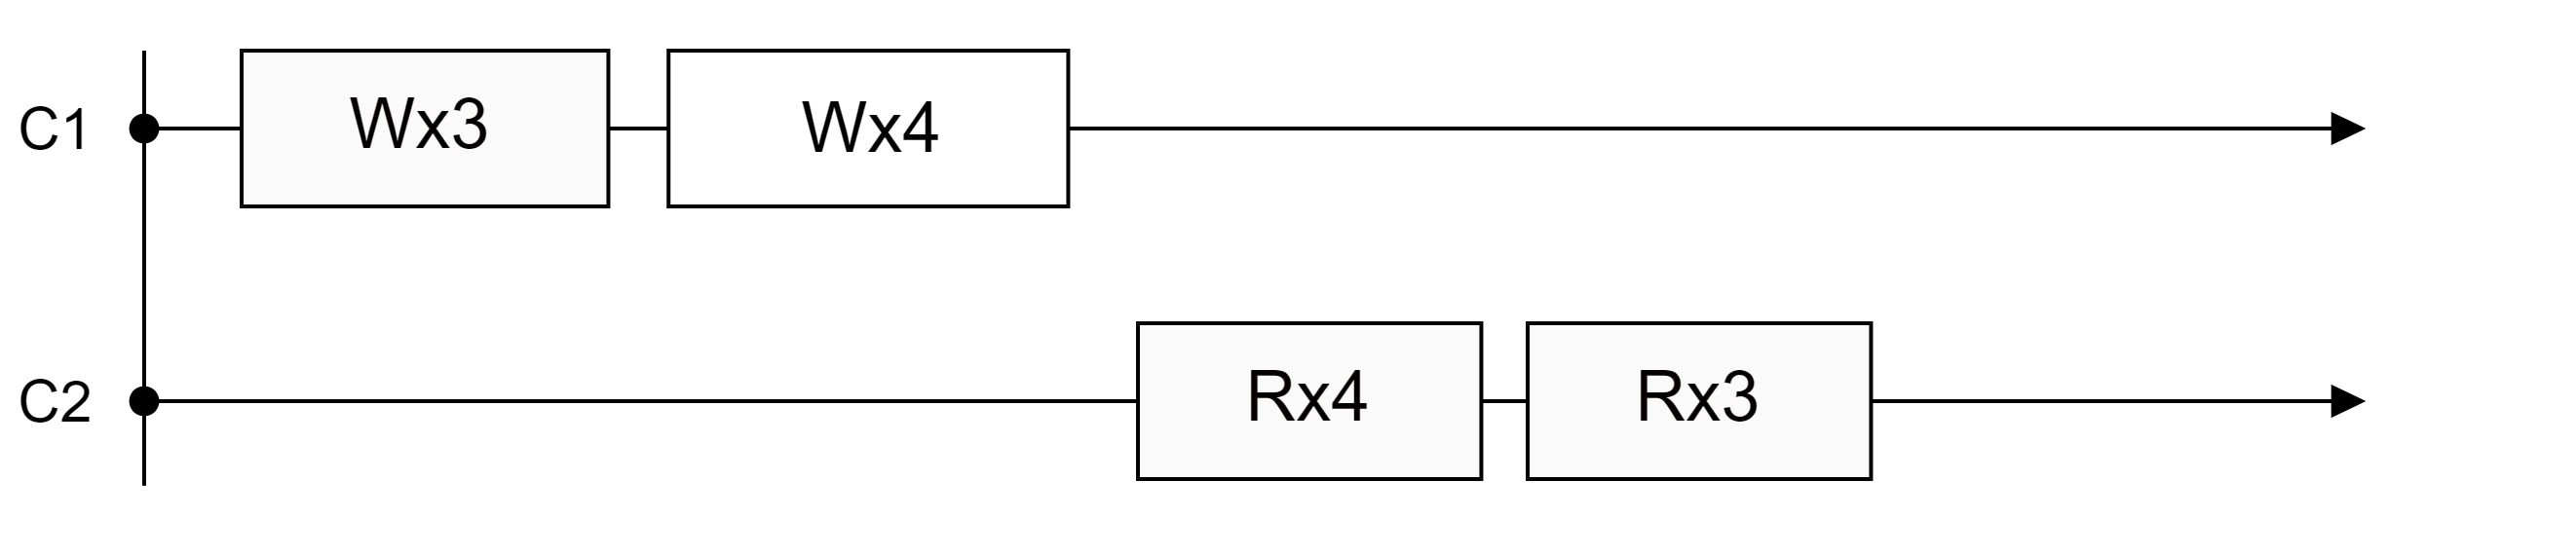
\includegraphics[width=.9\textwidth]{Sections/consist/fifo.png}
    \caption{This system is not FIFO nor Causally Consistent. Writes \textbf{must be read in monotonic order}. Hence, Rx3 must come before Rx4.}
\end{figure}

\begin{figure}[h]
    \centering
    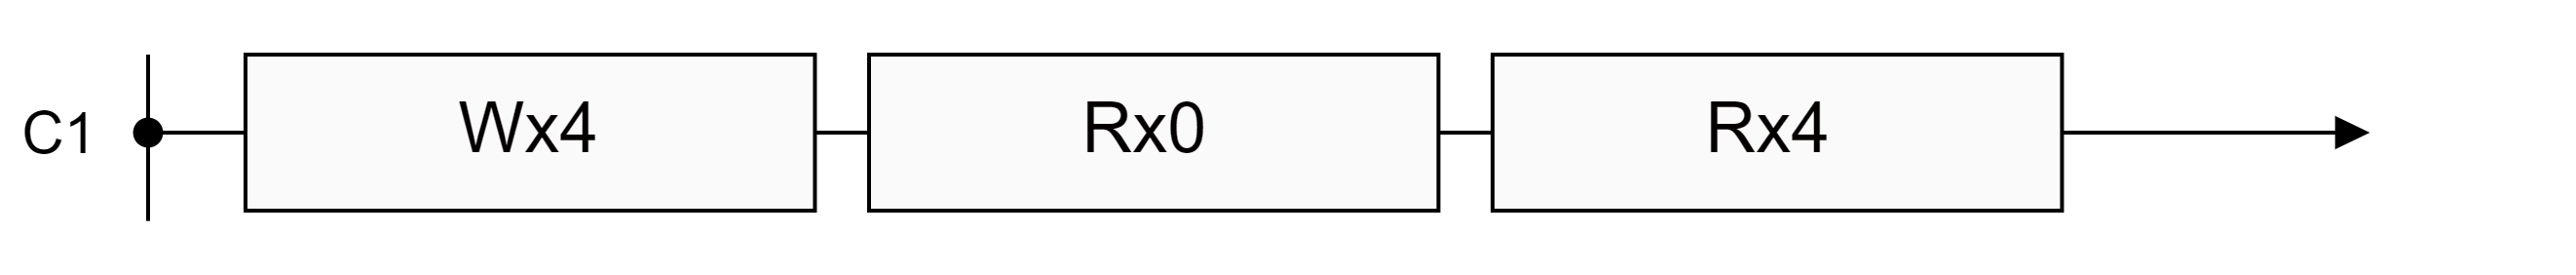
\includegraphics[width=.9\textwidth]{Sections/consist/ryw.png}
    \caption{This system is not RYW nor Causally Consistent. As the next read should be Rx4 alone. 
    The order, Rx0 $\rightarrow$ Wx4 $\rightarrow$ Rx4, satisfies RYW and is Causally Consistent.}
\end{figure}


    